\documentclass[12pt,spanish,letterpaper,color]{uchile}
\usepackage[ansinew]{inputenc}
\usepackage[spanish,activeacute]{babel}
\usepackage{anysize}
\usepackage{amsfonts}
\usepackage{float}
\usepackage{vmargin}
\usepackage{algorithm}
\usepackage{algorithmic}
\papersize{28.0cm}{21.5cm}
\setmarginsrb{3cm}{2cm}{2cm}{2cm}{\headheight}{\headsep}{\footheight}{\footskip}
\hyphenation{res-pec-ti-va-men-te mo-di-fi-can rea-li-dad fun-cio-na-li-da-des ma-llas re-fe-ren-cia-dos des-pla-za-mien-tos e-li-mi-nar che-quea-ba e-le-men-tos pos-te-rio-men-te  Lepp-Delaunay ma-lla co-li-nea-les vi-sua-li-zar}
\begin{document}

%% B. Nombre Institucion
\universidad{Universidad de Chile}
\facultad{Facultad de Ciencias F�sicas y Matem�ticas}
\departamento{Departamento de Ciencias de la Computaci�n}
%% C. Titulo
\title{Desarrollo de una herramienta que genera mallas de superficie compuestas de cuadril'ateros para modelar el crecimiento de 'arboles}
%% D. Proposito titulacion
\trabajoygrado{Memoria para optar al t�tulo de Ingeniero Civil en Computaci�n}
%% E. Autor
\author{Cristina Melo Lagos}
%% F. Profesores guia y comision
\profguia{Nancy Hitschfeld Kahler}
\profcom{Mar'ia Cecilia Rivara Z'u~niga}
\profco{Mar'ia Cecilia Rivara Z'u~niga}
\profint{Patricio Inostroza Fajardin}
%% G. Lugar y fecha
\ciudad{Santiago}
\pais{Chile}
\monthpub{Marzo}
\yearpub{2008}

\maketitle


%% Pagina optativa
%\section{Calificaciones}
%\makeeval

\begin{preface}




\begin{flushright}
	\begin{tabular}[t]{l}
	RESUMEN DE LA MEMORIA\\PARA OPTAR AL T'ITULO DE\\INGENIERO CIVIL EN COMPUTACI'ON \\
	POR: CRISTINA MELO LAGOS\\
	FECHA: 10/03/2008\\
	PROF. GU'IA: NANCY HITSCHFELD K.\\
	\end{tabular} 
\end{flushright}

\begin{center}
\begin{LARGE}
Desarrollo de una herramienta que genera mallas de superficie compuestas de cuadril'ateros para modelar el crecimiento de 'arboles
\end{LARGE}
\end{center}

El presente trabajo de t'itulo tuvo por objetivo desarrollar una herramienta para visualizar y modificar mallas de cuadril'ateros, que modelen la superficie del tronco de un 'arbol. Se enmarc'o dentro de un proyecto en el que dos alumnos hab'ian llevado a cabo su trabajo de t'itulo, por lo que el desarrollo consisti'o en extender la aplicaci'on existente.\\

El primer obst'aculo que se enfrent'o fue lograr un cabal entendimiento de la aplicaci'on del legado. Un aspecto que ayud'o a lograr este entendimiento fue el uso del paradigma de la Programaci'on Orientada a Objetos.\\

El trabajo se dividi'o en dos campos: dise~no e implementaci'on. En el primer 'ambito, se crearon jerarqu'ias de clases que modelaran la incorporaci'on de caras cuadril'ateras. Esto es, se crearon las jerarqu'ias \emph{Cara}, \emph{Tri'angulo} y \emph{Cuadril'atero} y \emph{Malla}, \emph{MallaTri'angulos} y \emph{MallaCuadril'ateros}.\\

Adem'as, se utiliz'o el patr'on \emph{AbstractFactory} para crear los algoritmos que modifican las mallas (deforman, refinan, desrefinan y mejoran), dependientes del tipo de caras que componen la malla.\\

En el 'ambito de la implementaci'on, se adaptaron los algoritmos existentes, o bien se crearon nuevos, para la generaci'on, guardado y deformaci'on de las mallas de cuadril'ateros.\\

Se implementaron m'etodos para convertir mallas de tri'angulos en mallas de cuadril'ateros y viceversa. Estos m'etodos permiten refinar y desrefinar mallas de cuadril'ateros, convirtiendo las caras en tri'angulos, aplicando luego los algoritmos para mallas de tri'angulos y aplicando otra conversi'on para tener una malla de cuadril'ateros.\\

El trabajo realizado cumple con el objetivo de poder trabajar con mallas de cuadril'ateros, aunque se requiere implementar m'as algoritmos para poder obtener un mayor provecho de la aplicaci'on. Se considera que el dise~no llevado a cabo otorga gran facilidad para la incorporaci'on de estos nuevos algoritmos.\\

%% Pagina optativa
\section{Agradecimientos}

Agradezco el apoyo prestado por la profesora gu'ia, Sra. Nancy Hitschfeld, durante el desarrollo de esta memoria. Su excelente disposici'on para atender mis dudas generaron interesantes discusiones que ayudaron a mejorar la calidad de este trabajo y, al mismo tiempo, propici'o un ambiente grato para este desarrollo.\\

Tambi'en debo mencionar mi agradecimiento a la Comisi'on Nacional de Investigaci'on Cient'ifica y Tecnol'ogica, CONICYT, por el financiamiento de este trabajo, a trav'es del proyecto Fondecyt -----.\\

Del mismo modo, agradezco a mi familia y amigos por el apoyo que me brindaron durante toda mi estad'ia en la universidad. En particular, a todos quienes compartieron conmigo durante el per'iodo en que se desarroll'o esta memoria.\\

%\section*{Tabla de contenidos}
\tableofcontents
%\listoftables
\listoffigures
%% Pagina optativa
%\section*{Indice de ilustraciones y cuadros}
\end{preface}
\chapter{Introducci�n}

\section{Antecedentes generales}

La Computaci'on Gr'afica abarca no s'olo desplegar figuras en la pantalla, sino que esas figuras sean el resultado del modelado de un problema real. Es as'i como una aplicaci'on com'un es tratar geom'etrica y num'ericamente un problema de compleja resoluci'on anal'itica. Para ello se requieren poderosas herramientas que permitan representar la realidad lo m'as fielmente posible, con las restricciones de factibilidad y costo computacional existentes.\\

Un ejemplo de lo anterior es el problema del crecimiento de un 'arbol. Existen trabajos anteriores \cite{ricardo, nicolas} en que, motivados por este problema, se construy'o una aplicaci'on que dada como entrada una malla geom'etrica triangular que representa el tronco de un 'arbol, modela su evoluci'on en el tiempo.\\

Por otra parte, las mallas de cuadril'ateros est'an siendo cada vez m'as comunes en aplicaciones tales como gr'afica de juegos, la industria del cine y visualizaciones m'edicas y cient'ificas.\\

Resulta entonces interesante comparar los resultados obtenidos utilizando una malla triangular y de cuadril'ateros, en el ejemplo antes descrito.\\

\section{Motivaci'on}

Se desea modelar el crecimiento de un 'arbol, en particular de la superficie 
cil'indrica de su tronco, mediante una malla de cuadril'ateros. Este modelamiento
permitir'a a otros profesionales estudiar esta discretizaci'on para luego 
extrapolar los resultados al modelo real.\\

El crecimiento del 'arbol se modela como el desplazamiento de cada uno de sus puntos,
 en direcci'on saliente al tronco. Por lo tanto, cada punto de la malla sufre distintos desplazamientos. La concentraci'on de la hormona de crecimiento en un punto es usada para estimar el desplazamiento de tal punto.
Es posible que al deformar la malla 'esta no quede consistente. Por ejemplo, pueden voltearse caras o intersectarse. Por lo tanto, surge la necesidad de abordar estrategias que se preocupen de mantener la consistencia de la malla al deformarla.\\

Adem'as, se requiere que la implementaci'on de la herramienta se adhiera al paradigma de la Programaci'on Orientada a Objetos, con el fin de apoyar la extensibilidad y claridad de la aplicaci'on a desarrollar, caracter'isticas muy valiosas considerando que probablemente otras personas continuar'an trabajando en este sistema.\\

\section{Objetivo general}

El objetivo general de esta memoria es implementar una herramienta para visualizar, desplazar y trabajar (refinar/desrefinar, suavizar) mallas geom'etricas de cuadril'ateros. Se reutilizar'a el dise~no de las clases y la implementaci'on de la interfaz gr'afica de la aplicaci'on del legado \cite{nicolas}, en la medida de lo posible. Se redise~nar'an clases y parte de la interfaz que necesiten perfeccionarse y se crear'an las clases necesarias para 
extender las funcionalidades de la aplicaci'on del legado a mallas de cuadril'ateros.\\

\section{Objetivos espec'ificos}

\begin{itemize}
\item Adaptar, dise~nar e implementar algoritmos para generar, cargar, visualizar y guardar mallas de cuadril'ateros.
\item Revisar y mejorar el dise~no actual. Por ejemplo, la representaci'on de la malla es una clase que posee m'etodos que no corresponden al alcance de la malla y que pueden reimplementarse en otra clase.
\item Incorporar algoritmos de transformaci'on para mallas de cuadril'ateros: deformaci'on, refinamiento y desrefinamiento.
\end{itemize}
	
\chapter{Antecedentes}

\section{Marco te'orico}

En la generaci'on de mallas en 2D (dos dimensiones), los dos enfoques m'as comunes son utilizar tri'angulos o cuadril'ateros.\\

Los tri'angulos son los pol'igonos m'as simples y poseen importantes propiedades (por ejemplo, sobre el tama~no de sus lados, medianas y puntos notables) y relaciones con circunferencias (inscritas, circunscritas). Esta simplicidad y, a la vez, riqueza, hacen que los tri'angulos hayan sido la figura geom'etrica natural para crear mallas geom'etricas que discretizan figuras reales.\\

Por otra parte, los cuadril'ateros son figuras m'as complejas que los tri'angulos y, a diferencia de 'estos, pueden no estar completamente contenidos en un plano (utilizando la definici'on gen'erica de cuadril'ateros, que no exige que sean pol'igonos). Adem'as, su representaci'on es m'as compleja, pues dependiendo del orden en que se unen los cuatro puntos, se genera un cuadril'atero v'alido o bien pol'igonos no simples (con arcos cruzados).\\

Sin embargo, el uso de mallas compuestas por cuadril'ateros es un enfoque que ha ganado adeptos, pues se considera que estas mallas son m'as precisas y flexibles. Una dificultad de abordar este enfoque es que no existe abundante literatura al respecto como en el caso de las mallas de tri'angulos.\\

En particular, enfoc'andose en el problema a tratar en esta memoria, se cree que las mallas de cuadril'ateros podr'ian representar mejor la estructura de la corteza de un 'arbol, al ser la forma de las c'elulas m'as similar a esta figura geom'etrica, lo que permitir'ia simular la distribuci'on de la hormona de crecimiento en el 'arbol de manera m'as natural.\\

Existe un \emph{trade-off} entre los m'etodos de generaci'on autom'atica de mallas geo\-m\'e\-tri\-cas y los que requieren intervenci'on manual. Los primeros entregan una malla de menor calidad (errores en los bordes de la malla y mayor n'umero de nodos irregulares), por lo que a veces se descompone manualmente la geometr'ia en regiones antes de aplicar los m'etodos autom'aticos, lo que evidentemente conlleva mayor trabajo. Existen tambi'en enfoques intermedios que intentan aprovechar lo mejor de ambas alternativas: \emph{paving} \cite{paving}, que construye progresivamente la malla insertando filas de cuadril'ateros desde el contorno del objeto hacia el interior.\\

Por otra parte, independientemente de la figura geom'etrica usada para general la malla, existen propiedades que se deben garantizar, en particular cuando se evaluar'an modelos matem'aticos en la malla generada, como en el caso de esta memoria. Algunas de las consideraciones necesarias son \cite{apunte, delnotes}:

\begin{itemize}
\item Representar el dominio de la manera m'as exacta posible, acotando el error. Esto es particularmente importante en los bordes, pues las aplicaciones cient'ificas o ingenieriles suelen ser sensibles a cambios en ellos.
\item Considerar las restricciones impuestas por los m'etodos num'ericos
usados, principalmente para acelerar la convergencia de 'estos. Las restricciones
son:
\begin{itemize}
\item Ser conforme.
\item Satisfacer requisitos de densidad de puntos, usando la
menor cantidad de puntos posibles. (M'etodos de refinamiento).
\item Satisfacer criterios de calidad medidos en funci'on de 'angulos,
aspecto de radio, altura y 'area, entre otros.
\item Evitar 'angulos muy peque~nos. (M'etodos para mejorar la calidad).
\end{itemize}
\end{itemize}

A continuaci'on se desarrollar'an alguno de estos puntos.\\

\subsection{Precisi'on en computaci'on geom'etrica}
%%%%%%%%%%%%%%%%%%%%%%%%%% ACORTAR %%%%%%%%%%%%%%%%%%%%%%%
Los computadores tienen recursos limitados y, por lo tanto, no pueden representar un conjunto infinito de n'umeros, como los enteros o los reales, sino que utilizan representaciones aproximadadas de 'estos. En el caso de los enteros, se representa s'olo un rango de ellos. En el caso de los reales, adem'as de no representar los valores fuera de un cierto intervalo, tampoco se representan todos los valores de ese intervalo, pues dentro de cualquier intervalo no vac'io de reales hay infinitos valores y obviamente no pueden representarse todos ellos. En adelante se limitar'a la discusi'on a la representaci'on de reales, tambi'en llamada \emph{representaci'on en punto flotante}, pues la Computaci'on Geom'etrica utiliza  a\-rit\-m\'e\-ti\-ca real y no entera.\\

El conjunto de n'umeros de punto flotante $\mathbb{F}(\beta, p, e_{min}, e_{max})$ se define como \cite{precision}:
$$\mathbb{F} = \{x = s \cdot \sum_{k=0}^{p-1} d_k \beta^{-k} \cdot \beta^e / s \in \{1,-1\}, d_k \in \mathbb{Z} \cap [0,\beta), $$
$$e \in \mathbb{Z} \cap [e_{min}, e_{max}], \sum |d_k| > 0 \Rightarrow d_0 > 0\}$$

La expresi'on anterior corresponde a la representaci'on normalizada, es decir, $d_0 > 0$ a menos que $x = 0$. Esta convenci'on se ocupa para disminuir los errores cometidos al realizar operaciones. En los sistemas computacionales, se trabaja con n'umeros binarios ($\beta = 2$) normalizados, por lo que $d_0$ es siempre 1, as'i que no es necesario almacenarlo.\\

Para aproximar n'umeros reales en este conjunto $\mathbb{F}$, se implementa la funci'on $fl: \mathbb{R} \rightarrow \mathbb{F}$, que a cada $x$ en $\mathbb{R}$ le asigna el n'umero en $\mathbb{F}$ m'as cercano a $x$ y de no ser 'unico, le asigna aqu'el con 'ultimo d'igito distinto de cero par.\\

El error relativo de aproximar $x$ por $fl(x)$ est'a acotado superiormente por $\epsilon_m$, una expresi'on constante con respecto a $x$ y dependiente s'olo de la base $\beta$ y de la mantiza $p$ caracter'isticas del conjunto $\mathbb{F}$. A esta expresi'on se le llama \emph{epsilon m'aquina}.\\

Los n'umeros representables en un sistema de punto flotante no se distribuyen homog'eneamente, sino que la distancia entre ellos va aumentando con el exponente $e$ utilizado; por lo tanto, aumenta el error absoluto que se puede cometer, pero el error relativo siempre est'a acotado por epsilon m'aquina.\\

Para implementar una funci'on real $f$ en un sistema de n'umeros flotantes, se construye una funci'on an'aloga $\tilde{f}$ que va desde $\mathbb{F}$ a $\mathbb{F}$ y se dice que implementa bien a la original si corresponde a la mejor aproximaci'on posible en $\mathbb{F}$, es decir, si:
$$\tilde{f}(x) = fl(f(x))$$

La mayor'ia de las funciones no son bien implementadas en los sistemas num'ericos.
S'olo se garantiza que un n'umero peque~no de ellas lo sea, como las operaciones
elementales binarias (suma, resta, multiplicaci'on y divisi'on) y algunas unarias 
(como la ra'iz cuadrada). Las dem'as funciones que se derivan de ellas no siempre
est'an bien implementadas y, por lo tanto, los errores relativos en los c'alculos
pueden ser mayores a epsilon m'aquina. Adem'as, al realizar sucesivas operaciones,
aunque cada una de ellas por separado est'e bien implementada, se va acumulando 
el error y aumenta la cota del error. Las operaciones que se realizan en un 
sistema de n'umeros flotantes se dice que usan aritm'etica imprecisa.\\

Un caso que se ha estudiado particularmente es el error num'erico en una suma de t'erminos: $S = \sum_i a_i$. La cota al error cometido que se ha encontrado es directamente proporcional a epsilon m'aquina, al n'umero de t'erminos sumados y a un factor de amplificaci'on $A$:

$$A = \frac{\sum_{a_i > 0} a_i + \sum_{a_i < 0} -a_i}{\sum_{a_i > 0} a_i - \sum_{a_i < 0} -a_i}$$

Si $\sum_{a_i > 0} a_i \approx \sum_{a_i < 0} -a_i$, entonces $A \rightarrow +\infty$, lo que se conoce como la amplificaci'on de errores producida por diferencias de n'umeros cercanos.\\

Lo anterior no significa que necesariamente los errores crezcan al hacer diferencia de n'umeros cercanos, pues se trata de una cota superior, pero emp'iricamente se han observado casos en que se alcanzan valores cercanos a la cota, por lo que es altamente recomendable evitar usar expresiones donde aparezcan diferencias de n'umeros cercanos. Por ejemplo, muchas de esas expresiones pueden reescribirse para evitar esta situaci'on:\\

\begin{itemize}
\item $\sqrt{n+1} - \sqrt{n} = \frac{1}{\sqrt{n+1} + \sqrt{n}}$
\item $\frac{1}{n} - \frac{1}{n+1} = \frac{1}{n(n+1)}$\\
\end{itemize}

Al no acotar el error acumulado puede tenerse que el valor absoluto del error de a\-pro\-xi\-ma\-ci\'on cometido sea mayor al valor absoluto de la expresi'on, es decir, ``que el error se coma la expresi'on''.\\

El no controlar los errores num'ericos cometidos al implementar algoritmos geom'etricos, puede llevar a programas que se caen, se quedan en ciclos infinitos, o simplemente entregan resultados err'oneos.\\
 
La parte m'as cr'itica en la implementaci'on son las condiciones, pues ellas determinan el flujo de control del programa. La mayor'ia de ellas involucran desigualdades, las que pueden reformularse como preguntas sobre el signo de una expresi'on. El enfoque m'as com'un es utilizar un valor epsilon para suponer que un n'umero es suficientemente cercano a cero, si es menor a epsilon, y por lo tanto considerarlo como cero, lo que puede ser errado pues entre cero y epsilon hay valores representables en la aritm'etica imprecisa cuya aproximaci'on a cero es incorrecta. El principal problema de este enfoque es que, para simplificar, se elige por ensayo y error el valor de epsilon y se le considera constante en todos los c'alculos, sin tomar en cuenta el tama~no de los operandos involucrados.\\

Un mejor enfoque es realizar c'alculos exactos, es decir, procurar que todas las
decisiones hechas por el algoritmo sean correctas. Para ello, no es necesario que
todos los c'alculos se realicen con aritm'etica exacta, sino que basta con que 
los errores producidos no alteren las decisiones del algoritmo. La t'ecnica de 
\emph{floating point filter} apunta a esto mismo y consiste en identificar aquellos casos en que el error podr'ia llevar a una mala decisi'on, y s'olo en esos casos, reevaluar la expresi'on con alguna t'ecnica que permita asegurar que la decisi'on es corecta; por ejemplo, esa t'ecnica puede ser usar arim'etica exacta. Esto se justifica porque realizar aritm'etica exacta es caro y en ocasiones ni siquiera es posible hacerlo, por ejemplo, no es posible representar exactamente n'umeros irracionales en ning'un sistema computacional, pues tienen infinitas cifras.\\

Por ejemplo, la t'ecnica de \emph{floating point filter} se puede usar para determinar si un conjunto de puntos est'a dentro de una circunferencia de centro $(x_0, y_0)$ y radio $r$. Para ello hay que revisar si cada punto $(x,y)$ cumple con la condici'on $r^2 - (x-x_0)^2 + (y-y_0)^2 \geq 0$. Para los puntos que no se encuentran ``cerca'' del borde (tomando como escala el posible error cometido), no se requiere usar aritm'etica exacta. En cambio los puntos cercanos al borde de la circunferencia se pueden calcular con aritm'etica exacta, pues utilizando aritm'etica inexacta podr'ian clasificarse, incorrectamente, como dentro o fuera de la circunferencia.\\

Al implementar un algoritmo geom'etrico hay que tratar con especial cuidado los \emph{casos degenerados}. Los casos degenerados corresponden una configuraci'on l'imite de un problema geom'etrico tal que no es una entrada que los algoritmos que resuelven el problema est'an preparados para recibir. En ese sentido, constituyen excepciones del algoritmo, pues no se les puede aplicar el mismo procesamiento que para el resto de las entradas. Desde el punto de vista del c'alculo, esto se traduce en que cuando el algoritmo quiere testear el signo de una expresi'on, se encuentra con que la expresi'on vale cero y hay que definir qu'e hacer en ese caso, pues se esperaba clasificar la expresi'on como positiva o negativa. Los casos degenerados obligan a hacer implementaciones m'as complejas para tratar estas excepciones. Otro enfoque es convertir un caso degenerado en uno no degenerado, d'andole un signo a las expresiones que son cero.\\

Otro problema existente es cuando se utilizan epsilons y se puede clasificar como un caso degenerado uno que no lo es (un valor muy cercano a cero, pero distinto de cero).\\

Un ejemplo de caso degenerado es cuando se quiere trabajar con el tri'angulo formado por tres rectas no paralelas, pero las tres rectas se intersectan en un mismo punto. Al determinar la distancia entre los v'ertices del tri'angulo, se espera que el valor sea positivo, pero se obtiene un valor cero.\\
%%%%%%%%%%%%% FIN ACORTAR %%%%%%%%%%%%%%%%%%%%%%
\subsection{Generaci'on de mallas geom'etricas}

Todo pol'igono puede ser particionado en tri'angulos mediante la sucesiva adici'on de diagonales \cite{orourke}. Este simple proceso describe un algoritmo de generaci'on de mallas triangulares en 2D. Sin embargo, el algoritmo ampliamente usado es la triangulaci'on de Delaunay, que asegura un grado de calidad de la malla al maximizar el m'inimo 'angulo entre todas las posibles triangulaciones de un pol'igono. Esto lo logra exigiendo que cada tri'angulo cumpla el criterio de Delaunay, esto es, que su circunc'irculo (el c'irculo circunscrito en el tri'angulo) sea vac'io, es decir, sin v'ertices en su interior, como se muestra en el ejemplo de la figura \ref{fig:delaunay}. El mismo principio se aplica para triangular superficies en 3D.\\

\begin{figure}[htp]
\centering
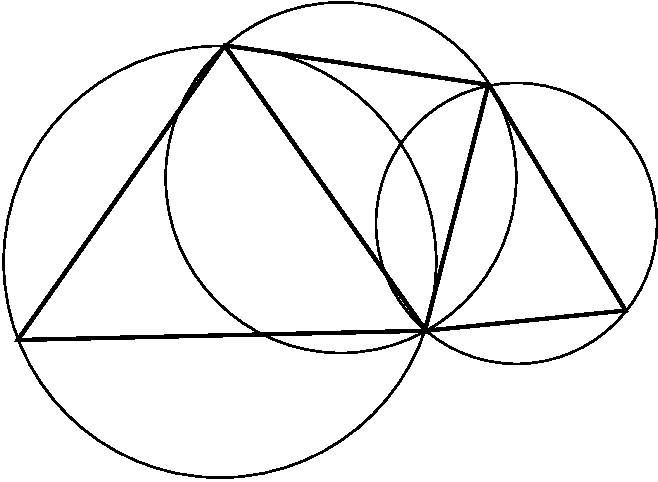
\includegraphics[scale=0.7]{img/delaunay.pdf}
\caption{Malla que cumple con el criterio de Delaunay}\label{fig:delaunay}
\end{figure}

En el caso de mallas de cuadril'ateros, pueden ser generadas triangulando el dominio y luego dividiendo cada tri'angulo en tres cuadril'ateros. Se puede incluso minimizar el n'umero de cuadril'ateros generados si el dominio es convexo. El problema de este enfoque es que puede generar mallas de mala calidad.\\

Otro enfoque es el presentado en \cite{cpack}, que apunta a ``empaquetar c'irculos'', esto es, llenar el dominio con c'irculos de modo que el espacio entre ellos est'e rodeado de tres o cuatro c'irculos tangentes y luego unir los centros de los c'irculos formando cuadril'ateros. Este algoritmo busca garantizar la calidad de la malla formada y acotar el n'umero de cuadril'ateros usados.\\

Un algoritmo que ha ganado adeptos es el de \emph{Paving} \cite{paving}, que permite generar mallas bien formadas (es decir, los elementos son cercanos a cuadrados, perpendiculares a los bordes, etc'etera) y geom'etricamente satisfactorias (es decir, los contornos de la malla tienden a seguir los contornos geom'etricos de los bordes).\\

El algoritmo consiste en iterativamente disponer filas de elementos desde el borde de la regi'on hacia el interior. Cuando las filas se superponen o coinciden, cuidadosamente se conectan para formar una malla de cuadril'ateros v'alida.\\

\begin{figure}[htp]
\centering
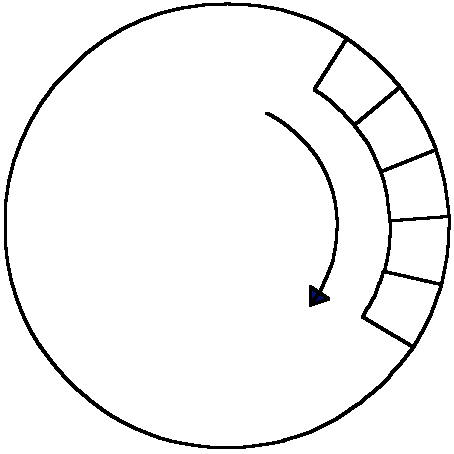
\includegraphics[scale=0.5]{img/img_1.pdf}
\caption{Algoritmo Paving}\label{fig:paving}
\end{figure}

Este algoritmo es un aporte con respecto a otros, pues logra generar una malla autom'aticamente, sin los costos comunes asociados a la automatizaci'on: mala calidad (falta de sensibilidad en los bordes y gran presencia de nodos que se conectan con un n'umero de nodos distinto a cuatro).\\

\section{Aplicaci'on del legado}

La aplicaci'on del legado corresponde al software desarrollado en dos memorias de t'itulo anteriores \cite{ricardo,nicolas}. A continuaci'on se describir'a el estado de la aplicaci'on al inicio del desarrollo de este trabajo de t'itulo.\\

\subsection{Funcionalidades}

La aplicaci'on trabaja con mallas de tri'angulos, pero tiene un desarrollo incipiente en mallas de cuadril'ateros.\\

En t'erminos generales, permite crear mallas simples, cargar mallas desde distintos formatos de entrada y guardarlas tambi'en en varios formatos de salida.\\

Permite la visualizaci'on gr'afica de mallas y modificar una malla deform'andola, refin'andola, desrefin'andola o mejor'andola. Adem'as, entrega informaci'on sobre la composici'on de la malla.\\

De forma m'as detallada, las funcionalidades de la aplicaci'on son:
\begin{description}
\item[Crear malla:] Se pueden crear mallas a partir de una m'edula y crear mallas cil'indricas. En el caso de la m'edula, el usuario especifica el nombre del archivo donde se encuentran las coordenadas de la m'edula. El cilindro, por su parte, corresponde al caso en que la m'edula es una vertical, por lo tanto, en vez de ingresarse las coordenadas de la m'edula, se ingresa la altura del cilindro. En ambos casos el algoritmo consiste en generar anillos horizontales alrededor de la m'edula. Cada anillo se compone de un n'umero constante de nodos. Al unir los nodos, se genera la malla. El usuario ingresa el radio, n'umero de anillos y n'umero de puntos por anillo que desea generar.

Las mallas cil'indricas pueden estar compuestas o bien de tri'angulos o bien de cuadril'ateros, seg'un lo decida el usuario. Las mallas generadas a partir de una m'edula s'olo son triangulares.

\begin{figure}[htp]
\centering
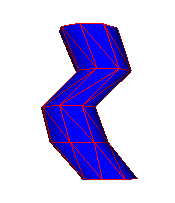
\includegraphics[scale=1.0]{img/img_2.png}
\caption{Malla triangular generada a partir de una m'edula}\label{fig:malla_medula}
\end{figure}

\item[Cargar malla:] Se pueden cargar mallas en distintos formatos de entrada: \emph{Comsol}, \emph{Matlab}, \emph{nxyzu} y \emph{Geomview} (los formatos se explican en el Ap'endice). Cada formato tiene su propio algoritmo para cargar la malla, pero a grandes rasgos todos ellos leen las coordenadas de los nodos de la malla, leen o deducen el orden en que los nodos forman las caras, crean los nodos y caras correspondientes y adem�s los arcos de las caras. Del mismo modo leen o calculan las normales de los puntos y calculan las normales de las caras. Una vez cargada la malla, ya no se distingue desde qu'e formato fue cargada, o si fue creada directamente en la aplicaci'on.

\item[Visualizar malla:] Al crear o cargar una malla, 'esta es dibujada por la aplicaci'on. Se puede elegir si se desean ver o no las caras y/o arcos de la malla. Adem'as, se puede mover la c'amara de forma de acercar, alejar y rotar la malla.

\item[Guardar mallas:] Las mallas pueden ser guardadas en distintos formatos de salida: \emph{Comsol}, \emph{nxyzu}, \emph{Off} y \emph{Debug}. Este 'ultimo formato es de uso interno y se utiliza para depurar la aplicaci'on, pues consiste en un recorrido exhaustivo por toda la informaci'on de la malla.

\item[Deformar malla:] La malla puede ser deformada. La deformaci'on consiste en el desplazamiento de cada nodo de la malla seg'un su concentraci'on y en direcci'on normal al nodo. El usuario indica el porcentaje de la concentraci'on que se mover'a cada nodo en un paso y el n'umero de pasos que se mover'a la malla. Los nodos se desplazan un paso por unidad de tiempo y se puede cambiar la velocidad de la animaci'on resultante. El usuario tambi'en ingresa el algoritmo de verificaci'on 	que desea aplicar, es decir, c'omo se tratar'an las posibles inconsistencias que se producir'an al desplazar los nodos de la malla. Uno de las opciones posibles en no realizar ninguna verificaci'on, es decir, deformar la malla aunque 'esta quede inconsistente.

\item[Refinar malla:] Se puede refinar la malla, es decir, aumentar el n'umero de caras de la malla disminuyendo el 'area de las caras originales. El usuario elige el algoritmo de refinamiento y el criterio de detenci'on del algoritmo.

\item[Desrefinar malla:] Se puede desrefinar la malla, es decir, disminuir el n'umero de caras de la malla aumentando el 'area de las caras sobrevivientes. El usuario elige el criterio de detenci'on del algoritmo de desrefinamiento.

\item[Mejorar malla:] Se puede aplicar un algoritmo de mejoramiento de la calidad de la malla. El algoritmo implementado es el que usa el criterio de Delaunay.

\item[Ver informaci'on malla:] Se puede desplegar un cuadro con informaci'on sobre la composici'on de la malla (n'umero de caras, 'area promedio de las caras, etc.). Esta informaci'on es de suma importancia para escoger los par'ametros adecuados al aplicar algoritmos de refinamiento y desrefinamiento.\\

\end{description}

\subsection{Dise~no}

La aplicaci'on del legado fue dise~nada siguiendo el paradigma de la Programaci�n Orientada a Objetos. En la figura \ref{fig:diagrama_clases_legado} se muestra el diagrama de clases, en donde se aprecia el uso de patrones de dise~no y la separaci'on entre la capa de presentaci'on y la l'ogica de la aplicaci'on.\\

\begin{figure}[htp]
\centering
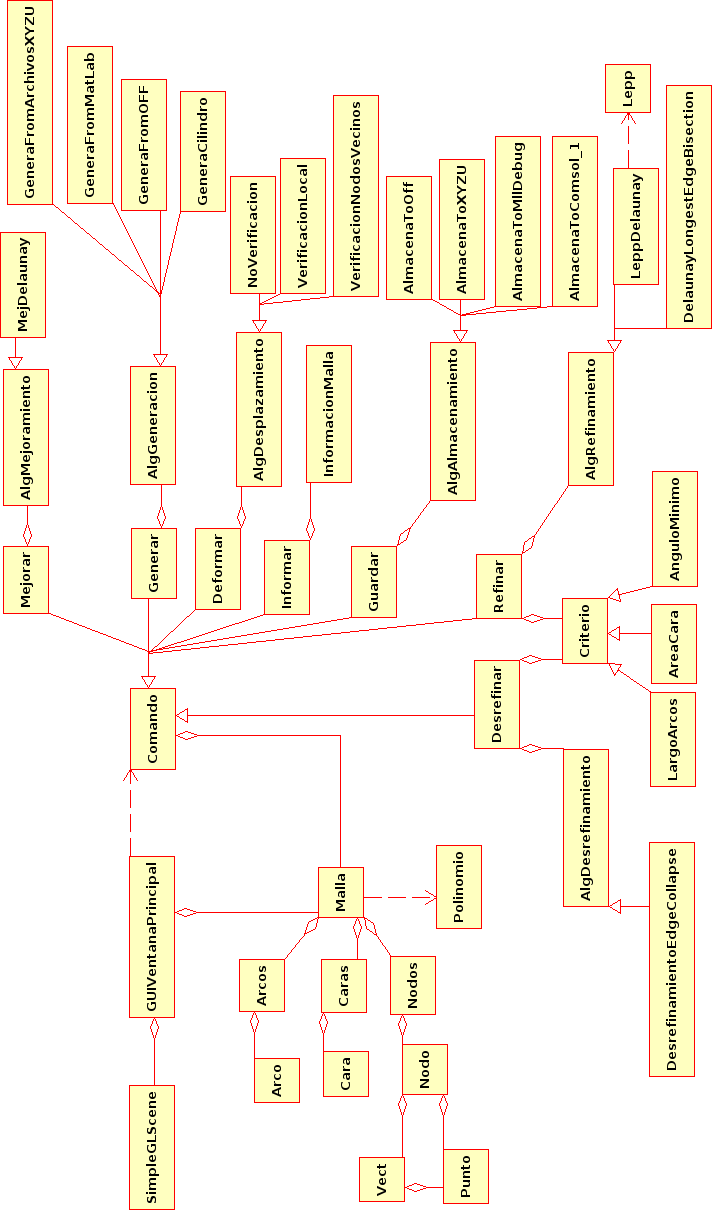
\includegraphics[scale=0.45]{img/diseno_legado.png}
\caption{Diagrama de clases de la aplicaci'on del legado}\label{fig:diagrama_clases_legado}
\end{figure}

Los patrones de dise~no entregan buenas soluciones a problemas recurrentes en el dise~no de un sistema,
beneficiando particularmente la reusabilidad del sistema. A continuaci'on se describen los patrones utilizados en la aplicaci'on del legado.

\begin{description}
\item[Command:] En la aplicaci'on, este patr'on es utilizado para encapsular los requerimientos que el usuario realiza a trav'es de la interfaz gr'afica, de modo de separarlos de la capa l'ogica que se encarga de ejecutarlos. Las clases que cumplen el rol de comandos son \emph{Generar}, \emph{Guardar}, \emph{Refinar}, \emph{Desrefinar}, \emph{Mejorar}, \emph{Desformar} e \emph{Informar}.
\item[Strategy:] Este patr'on es utilizado para encapsular una familia de algoritmos de forma que sea f'acil intercambiarlos y agregar nuevos algoritmos. En la aplicaci'on, para cada comando, salvo \emph{Informar}, hay una familia de algoritmos encargada de satisfacer el requerimiento asociado al comando.

Este patr'on es muy 'util en una aplicaci'on como 'esta, donde distintas personas han trabajado en distintas iteraciones, pues la incorporaci'on de un nuevo algoritmo se limita a la creaci'on de la clase que lo implementa y
a agregar la opci'on en la interfaz.

\end{description}

Se considera que hay dos importantes aspectos mejorables del dise~no. El primero es la clase \emph{Cara}, que representa una cara de cualquier n'umero de lados, pero que tiene m'etodos que s'olo son v'alidos para tri'angulos. El segundo es la clase \emph{Malla}, que tiene m'as de 50 m'etodos p'ublicos, sin contar constructores, \emph{setters} ni \emph{getters}. Esto se debe a que la malla es la 'unica clase que tiene toda la informaci'on necesaria para realizar la mayor�a de los c'alculos necesarios, situaci'on que se explicar'a en m'as detalle en la pr'oxima secci'on.\\

La gran cantidad de m'etodos de la clase \emph{Malla} es un problema, pues afecta su mantenibilidad y adem'as es conceptualmente errado que esa clase deba hacerse cargo de comportamientos que no le corresponden, como determinar el 'area de una cara.

\subsection{Representaci'on de la malla}

A continuaci'on se explica la representaci'on de la clase \emph{Malla}, la m'as importante del sistema y, a su vez, la representaci'on de las clases que la componen.\\

\begin{description}
\item[Malla:] B'asicamente, se representa por tres contenedores: de objetos nodos, arcos y caras.

\item[Nodo:] Se representa mediante un punto, un vector normal y una concentraci'on. Por razones de eficiencia, mantiene adem'as vectores de 'indices de los arcos y caras de los que forma parte. Los 'indices, tanto en esta clase como en las siguientes, son con respecto a los contenedores que almacena la malla.

\item[Arco:] Se representa mediante 'indices de los dos nodos que lo conforman y de las dos caras de las que forma parte.

\item[Cara:] Se representa mediante vectores de 'indices de los nodos y arcos que la conforman. Adem'as, almacena su n'umero de lados y color.

\end{description}

La aplicaci'on trabaja con clases contenedoras: \emph{Nodos}, \emph{Arcos} y \emph{Caras}, que proveen m'etodos para borrar, agregar y obtener elementos, entre otros m'etodos.\\

De lo anterior se deduce que s'olo la clase \emph{Malla} tiene referencias a los nodos, arcos y caras. Las otras clases almacenan 'indices, pero no tienen acceso a los contenedores referenciados por los 'indices. Por lo tanto, un arco no es capaz de calcular su largo, pues no conoce la posici'on de los nodos que lo forman, sino s'olo los 'indices de los nodos. Esto hace que las clases \emph{Nodo}, \emph{Arco} y \emph{Cara} est'en compuestas principalmente por constructores, \emph{setters} y \emph{getters} y que los comportamientos de estas clases est'en implementados en la clase \emph{Malla}.\\

\subsection{Algoritmos}

La aplicaci'on implementa una serie de algoritmos para modificar la malla. A con\-ti\-nua\-ci\'on se explican.

\begin{description}
\item[Verificaci'on desplazamiento:] Al deformar la malla, cada nodo se desplaza una distancia proporcional a su concentraci'on, en la direcci'on de su normal. Estos desplazamientos pueden producir colisiones, por lo que se implementan tres algoritmos para tratarlas: \emph{No Verificaci'on}, \emph{Verificaci'on Local} y \emph{Verificaci'on Nodos Vecinos}. El primero de ellos no realiza ninguna verificaci'on, por lo que simplemente desplaza la malla.

El algoritmo \emph{Verificaci'on Local} recorre pares de caras vecinas (comparten un arco) coplanares y detecta si hay intersecci'on entre sus arcos y, de haberla, intenta corregir esta inconsistencia haciendo \emph{flipping} de arcos.

El algoritmo \emph{Verificaci'on Nodos Vecinos} recorre los nodos y para cada nodo, encuentra el pol'igono formado
por los arcos de las caras incidentes en el nodo, de forma que el nodo queda en el centro del pol'igono. Luego,
construye un pseudocilindro en que la base inferior es el pol'igono y la base superior est'a formada por las
posiciones futuras de los v'ertices del pol'igono (luego del desplazamiento), de forma tal que las aristas
verticales del cilindro son las trayectorias de los v'ertices. El algoritmo determina si la trayectoria del nodo
central colisiona con alguna de las paredes del cilindro, lo que provocar'ia que una cara se volteara. Si es as'i,
corrige la trayectoria del nodo central, haciendo que la direcci'on de la normal del nodo sea la suma de las
normales de los v'ertices del pol'igono. Si este proceso no corrige la inconsistencia, entonces borra el nodo
central.

\item[Refinamiento:] Existen dos clases que implementan algoritmos de refinamiento: \emph{LeppDelaunay} y 
\emph{DelaunayLongestEdgeBisection}. En la primera de ellas se aplica el algoritmo \emph{LEPP-Delaunay} \cite{leppdelaunay} a cada cara que no cumple con el criterio dado. El algoritmo \emph{LEPP-Delaunay} iterativamente encuentra el 
\emph{LEPP} (\emph{Longest Edge Propagation Path}) de la cara a refinar y realiza una inserci'on \emph{Delaunay} en
la arista terminal, es decir, divide los dos tri'angulos unidos por la arista y hace \emph{flipping} de arcos
para que cumplan el criterio de \emph{Delaunay}, en caso que fuera necesario.

En la segunda clase, \emph{DelaunayLongestEdgeBisection}, en cada cara que no cumple el criterio, se divide 
por la mitad su arco m'as largo, cambiando los arcos necesarios para que se cumpla el criterio de \emph{Delaunay}
antes y despu'es de la divisi'on.

\item[Desrefinamiento:] El algoritmo \emph{Desrefinamiento Edge Collapse} recorre la malla buscando caras que no cumplan el criterio de detenci'on. Luego detecta el menor arco de esa cara y lo colapsa en un nodo, eliminando las dos caras adyacentes a 'el.

\item[Mejora:] El algoritmo \emph{Mejora Delaunay} recorre la malla buscando pares de tri'angulos vecinos que no cumplan el criterio de Dalaunay (es decir, existen v'ertices al interior del c'irculo circunscrito en 'el). Luego reemplaza el arco com'un de los tri'angulos por el otro posible, haciendo que ambos tri'angulos cumplan con el criterio (\emph{flipping} de arcos).

\end{description}

\chapter{Dise~no}

\section{Redise~no asociado a la incorporaci'on de mallas de cuadril'ateros}

Para incorporar a la aplicaci'on mallas de cuadril'ateros se hace necesario modificar la clase \emph{Cara}. En la aplicaci'on del legado, esta clase est'a representada por vectores de 'indices de nodos y de arcos y por un entero que indica el n'umero de lados de la cara.\\

El trabajar con vectores sin preocuparse de su largo, es decir, del n'umero de lados de la cara, hace que los m'etodos sean m'as generales y por lo tanto m'as reusables. Adem'as, en muchos casos acortan la extensi'on del c'odigo. Sin embargo, es incorrecto conceptualmente tener las caras de cualquier n'umero de lados en una misma clase siendo que no tienen siempre el mismo comportamiento, lo que se evidencia en la implementaci'on del legado en que hay m'etodos de la clase que s'olo son v'alidos para tri'angulos.\\

La necesidad de crear una jerarqu'ia se hace m'as clara a'un al querer extender los algoritmos de desplazamiento, refinamiento, desrefinamiento y mejoramiento a mallas de cuadril'ateros. Estos algoritmos son fuertemente dependientes de la forma de las caras de la malla y, por lo tanto, no es cierto que funcionen para caras de cualquier n'umero de lados. Por ejemplo, el algoritmo de mejoramiento utiliza el \emph{criterio de Delaunay}, que se basa en propiedades geom'etricas de los tri'angulos.\\

Corresponde entonces crear una jerarqu'ia para la clase \emph{Cara} donde ella es la clase base y las clases \emph{Tri'angulo} y \emph{Cuadril'atero} son derivadas, dejando adem'as abierta la posibilidad a la incorporaci'on de nuevas clases (caras con m'as de cuatro lados).\\

El primer enfoque que se tom'o para llevar a cabo este redise~no fue hacer que la clase \emph{Cara} fuera una clase abstracta que incluyera todos los m'etodos que representan el comportamiento de una cara, independientemente de su n'umero de lados. Los m'etodos que representan el comportamiento espec'ifico de un tri'angulo o cuadril'atero, deb'ian estar en su correspondiente clase derivada.\\

Este enfoque finalmente fue modificado pues algunos de los formatos desde los que se carga la malla soportan el uso de caras de m'as de cuatro lados y los archivos de ejemplo con los que se trabaja incluyen esos casos. Se prefiri'o entonces no restringir la aplicaci'on y seguir permitiendo la visualizaci'on de este tipo de mallas, aunque no exista la implementaci'on de los algoritmos para modificar esas mallas. Por lo tanto, se decidi'o que la clase \emph{Cara} no ser'ia abstracta, sino que se crear'ian instancias para representar caras de m'as de cuatro lados y que los algoritmos que modifican la malla y que son propios de tri'angulos o cuadril'ateros trabajar'ian con objetos de la clase derivada correspondiente, de forma de mantener la correctitud conceptual de la aplicaci'on.\\

Del mismo modo, se hizo necesario crean una jerarqu'ia para la clase \emph{Malla}, por lo que se crearon las clases \emph{MallaTri'angulos} y \emph{MallaCuadril'ateros} y se permiti'o igualmente tener instancias de la clase \emph{Malla} original.\\

Se deseaba hacer un dise~no que permitiera trabajar con mallas de tri\-\'an\-gu\-los y cua\-dri\-l\'a\-te\-ros lo m'as transparentemente posible, de forma de asociar correctamente los algoritmos v'alidos a cada tipo de malla, sin tener que hacer chequeos de tipo. Tambi'en se con\-si\-de\-r\'o importante facilitar la incorporaci'on de nuevos tipos de malla, por ejemplo, una malla mixta de tri'angulos y cuadril'ateros.\\

Se decidi'o utilizar el patr'on \emph{Abstract Factory} \cite{oop} para que la elecci'on de los tipos de algoritmos a utilizar se realizara una sola vez, al crear la f'abrica, y que luego el resto de la implementaci'on pudiera abstraerse del tipo de malla con la cual se estaba trabajando. Con este enfoque, se crear'ian dos f'abricas, una para los algoritmos aplicables en mallas de tri'angulos y otra para los aplicables en mallas de cuadril'ateros. Los productos ser'ian los algoritmos para desplazar, refinar, desrefinar y mejorar las mallas.\\

El problema que surgi'o es que para cada una de estas acciones que pueden realizarse sobre la malla, existe potencialmente una familia de algoritmos que las lleva a cabo, pues se est'a usando el patr'on \emph{Strategy}. Por lo tanto existen dos jerarqu'ias que deben convivir: la que refleja el tipo de malla en el que el algoritmo se aplica y la que refleja las distintas implementaciones existentes para el algoritmo. Se evalu'o utilizar el patr'on \emph{Bridge} para dise~nar esta situaci'on, pero se consider'o que no era aplicable porque la implementaci'on del algoritmo depende del tipo de malla en que se usa.\\

La soluci'on llevada a cabo fue hacer una doble jerarqu'ia para cada tipo de algoritmo. Primero se divide seg'un el tipo de malla sobre el que se aplica el algoritmo y luego se hace la divisi'on seg'un las implementaciones. La opci'on de hacer las jerarqu'ias en el orden inverso, es decir, primero por implementaci'on y luego por tipo de malla, se descart'o pues no todas las implementaciones existen para cada tipo de malla. En cambio, conceptualmente pueden existir implementaciones para cada tipo gen'erico de algoritmo, para cada tipo de malla.\\

Para incorporar el patr'on \emph{Abstract Factory} se consider'o s'olo la primera jerarqu'ia de cada tipo de algoritmo, pues el patr'on es aplicable si se pueden fabricar los mismos tipos de productos en cada f'abrica. Como se dijo anteriormente, los productos no pueden ser las implementaciones espec'ificas de cada algoritmo, pues la f'abrica de mallas de tri'angulos no ofrecer'ia los mismos productos (implementaciones) que la f'abrica de mallas de cuadril'ateros.\\

Finalmente, el dise~no adoptado se muestra en la figura \ref{fig:abstractfactory}, donde se observa que cada m'etodo de la f'abrica recibe un identificador del tipo de implementaci'on que se elegir'a, seg'un la segunda jerarqu'ia creada para cada algoritmo. Se puede ver un ejemplo del m'etodo para crear un algoritmo de desplazamiento en la f'abrica de mallas de tri'angulos y en la de cuadril'ateros, en \emph{Algorithm \ref{codigo_abstract_factory_t}} y \emph{Algorithm \ref{codigo_abstract_factory_q}}, respectivamente.\\

\begin{figure}[htp]
\centering
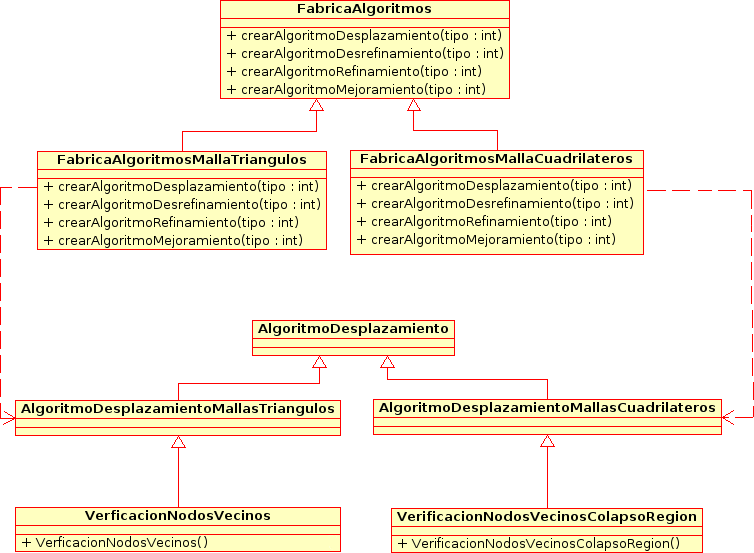
\includegraphics[scale=0.6]{img/abstractfactory.png}
\caption{Diagrama de clases para la creaci'on de algoritmos de desplazamiento}\label{fig:abstractfactory}
\end{figure}

\begin{algorithm}
\caption{Creaci'on de algoritmo desplazamiento en \emph{FabricaAlgMallaTri'angulos}} \label{codigo_abstract_factory_t}
\begin{algorithmic} [1]
\STATE AlgDesplazamiento *crearAlgoritmoDesplazamiento(int tipo) $\{$
\STATE AlgDesplazamientoMallaTriangulos *algoritmo = NULL
\IF{tipo = 1}
\STATE algoritmo = new NoVerificacion()
\ELSIF{tipo = 2}
\STATE algoritmo = new VerificacionLocal()
\ELSIF{tipo = 3}
\STATE algoritmo = new VerificacionNodosVecinos()
\ENDIF
\RETURN algoritmo
\STATE $\}$
\end{algorithmic}
\end{algorithm}

\begin{algorithm}
\caption{Creaci'on de algoritmo desplazamiento en \emph{FabricaAlgMallaCuadril'ateros}} \label{codigo_abstract_factory_q}
\begin{algorithmic} [1]
\STATE AlgDesplazamiento *crearAlgoritmoDesplazamiento(int tipo) $\{$
\STATE AlgDesplazamientoMallaCuadrilateros *algoritmo = NULL
\IF{tipo = 1}
\STATE algoritmo = new VerificacionNodosVecinosColapsoRegion()
\ENDIF
\RETURN algoritmo
\STATE $\}$
\end{algorithmic}
\end{algorithm}

El crear estas jerarqu'ias implic'o trabajar en varios 'ambitos. El primero fue revisar todos los m'etodos de las clases a especificar (\emph{Cara} y \emph{Malla}) e identificar los m'etodos que implementaban comportamientos propios de esas clases gen'ericas, modificando sus implementaciones en los casos que fue necesario, como cuando hab'ia implementaciones v'alidas s'olo para tri'angulos, pero que eran generalizables. Adem'as, se dejaron en las subclases los m'etodos espec'ificos, tanto los existentes como los que hubo que implementar para caras y mallas de cuadril'ateros.\\

Otro 'ambito a abordar fue el detectar la creaci'on de objetos de las clases bases y cambiarlos por la creaci'on de objetos de las subclases, seg'un correspondiera.\\

\section{Redise~no de la clase Malla}

Esta clase necesitaba ser redise~nada pues pose'ia m'as de 50 m'etodos p'ublicos, sin contar los contructores, \emph{getters} y \emph{setters}. Esta gran cantidad de m'etodos le quitaba mantenibilidad a 'esta, la principal clase del sistema.\\

Esta gran cantidad de m'etodos se debe a la representaci'on de la malla, explicada anteriormente, que hac'ia que esta clase fuera la 'unica que pod'ia implementar comportamientos propios de las clases \emph{Nodo}, \emph{Arco} o \emph{Cara}.\\

Se evalu'o la posibilidad de cambiar la representaci'on de las clases \emph{Malla}, \emph{Nodo}, \emph{Arco} y \emph{Cara}. Sin embargo, esta idea se descart'o por el costo y riesgo de hacer un cambio tal magnitud en la aplicaci'on y porque los motivos de eficiencia que llevaron a trabajar con contenedores e 'indices siguieron pesando. Entonces, se decidi'o mantener la representaci'on y cambiar los m'etodos cuestionados a las clases correspondientes, agreg'andoles como argumento la malla. Es decir, los m'etodos reciben la malla como par'ametro y pueden pedirle la informaci'on que necesiten para implementar los comportamientos requeridos. Por ejemplo, la clase \emph{Arco} ahora implementa el m'etodo para calcular su largo, pidi'endole a la malla los objetos \emph{Nodo} que  componen el arco, para poder obtener la posici'on de 'estos.\\

De esta forma, aumenta el acoplamiento de las clases \emph{Nodo}, \emph{Arco} y \emph{Cara} con la clase \emph{Malla}, pues estas clases requieren de esta 'ultima para implementar sus comportamientos. Sin embargo, se considera que este punto es inevitable, pues refleja la realidad en la que estos elementos geom'etricos efectivamente est'an acoplados.\\

Uno de los motivos que dificultaba el cambio en la representaci'on de la malla era la existencia de m'etodos p'ublicos que obten'ian los contenedores de nodos, arcos y caras. De este modo, se perjudicaba la independencia entre la representaci'on de la clase y sus usuarios. Para mejorar este aspecto, se reemplazaron tales m'etodos por otros para obtener un nodo, arco o cara particular, y no su contenedor. De esta forma, para iterar sobre los nodos de la malla se le pide iterativamente cada nodo, sin comprometer la privacidad de la implementaci'on.\\

\chapter{Implementaci'on}

Como se explic'o anteriormente, la creaci'on de las jerarqu'ias de la clases \emph{Cara} y \emph{Malla} tuvo amplias repercusiones en el c'odigo de la aplicaci'on, implicando cambiar la implementaci'on existente y agregar nuevos algoritmos. A continuaci'on se explica c'omo se llev'o a cabo en cada una de las partes relevantes de la aplicaci'on.\\

\section{Generaci'on de malla}

La malla puede ser generada desde una m'edula ingresada por el usuario, o generada en forma cil'indrica. Para el caso de la malla cil'indrica, la aplicaci'on del legado ten'ia implementada la opci'on con mallas de cuadril'ateros, as'i es que s'olo hubo que cambiar la creaci'on de los objetos de la clase \emph{Cara} por objetos de las clase \emph{Tri'angulo} o \emph{Cuadril'atero} y la creaci'on de los objetos de la clase \emph{Malla} por objetos de las clase \emph{MallaTriangulos} o \emph{MallaCuadril'ateros}, seg'un correspondiera.\\

La generaci'on de la malla a partir de una m'edula se extendi'o para el caso de mallas de cuadril'ateros. Para esto, primero se modific'o la interfaz para permitir la elecci'on entre una malla de tri'angulos y una de cuadril'ateros. Luego se agreg'o un m'etodo que genera la malla de cuadril'ateros. El algoritmo consiste en generar los anillos de la malla desde abajo hacia arriba. Al tener un anillo, se itera sobre el n'umero de puntos del anillo. Para cada punto, se reconocen cuatro nodos: el actual, el siguiente en el mismo anillo, el superior al actual y el superior al siguiente del actual, como se muestra en la figura \ref{fig:medula_Cuadril'atero}. Con esos nodos se crea el cuadril'atero, creando tambi'en los correspondientes arcos.\\

\begin{figure}[htp]
\centering
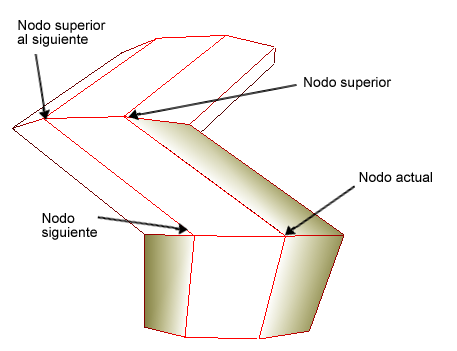
\includegraphics[scale=0.5]{img/img_3.png}
\caption{Generaci'on de caras cuadril'ateras a partir de una m'edula}\label{fig:medula_Cuadril'atero}
\end{figure}

\section{Carga de malla}

La malla puede ser cargada en cuatro formatos, para todos ellos hay que adaptar el algoritmo de lectura para que trabaje tambi'en con mallas de cuadril'ateros.\\

En el caso del formato \emph{Matlab} ya exist'ia un m'etodo para cargar mallas de cuadril'ateros. El formato almacena nodos y su ubicaci'on en anillos alrededor de una m'edula impl'icita, por lo que un mismo archivo puede representar una malla de tri'angulos o de cuadril'ateros, dependiendo de c'omo se unen los nodos mediante arcos. Es por esto que el usuario elige el tipo de malla a crear a partir de un archivo en este formato. La aplicaci'on del legado ya ten'ia implementada esta funcionalidad, pero se detect� y solucion'o un error que dejaba la malla inconsistente (m'as adelante se detallar�).\\

En el caso de los otros formatos, la estrategia usada fue generalizar el algoritmo existente, en vez de crear otro para el caso de cuadril'ateros. De esta forma, se evita duplicar el c�digo y por lo tanto se ayuda a la mantenibilidad de la aplicaci'on. La generalizaci'on consisti� en detectar el c�digo com�n para ambos tipos de cara, dejarlo parametrizado con respecto al n�mero de lados (tres 'o cuatro) y separar las partes diferentes seg�n el tipo de cara, por ejemplo, la creaci�n del objeto \emph{Tri'angulo} o \emph{Cuadril'atero}.\\

El formato \emph{Geomview} ya estaba generalizado y ahora se crean objetos \emph{Tri'angulo}, \emph{Cuadril'atero} o \emph{Cara} seg�n si el n'umero de lados de la cara es tres, cuatro o mayor, respectivamente.\\

En los formatos \emph{Comsol} y \emph{nxyzu} la generalizaci�n es v�lida para caras triangulares y cuadril'ateras. No se consider'o necesario extenderlo tambi'en a caras de m'as lados, pues ese caso no se presenta en las mallas de ejemplo que se tienen (a diferencia del formato \emph{Geomview}), pero se considera que ya hecha esta primera generalizaci'on, las posteriores no presentan gran dificultad.\\

Para estos dos �ltimos formatos se dej'o tambi'en la opci'on de que la malla sea mixta, es decir, que est'e formada por caras triangulares y cuadril'ateras. Sin embargo, al igual que en el caso de caras de m'as de cuatro lados, la aplicaci'on no provee algoritmos para modificar esas mallas, por lo que s'olo pueden ser visualizadas.\\

\section{Guardado de malla}

Para cada uno de los cuatro formatos de salida de la malla fue necesario adaptar los algoritmos de guardado para que iteraran sobre los nodos y arcos sin suponer que su cardinalidad era tres. Adem'as, en el caso de los formatos \emph{Comsol} y \emph{nxyzu} se cubri'o el caso en que la malla es mixta.\\

\section{Algoritmo de eliminaci'on de un nodo}

La eliminaci'on de un nodo de la malla es una operaci'on que la aplicaci'on del legado utiliza al deformar la malla, cuando se produce una inconsistencia que no puede ser reparada cambiando el vector normal del nodo (como se explic'o en la secci'on 2.2.4). Adem'as se utiliza para desrefinar la malla.\\

El algoritmo para tri'angulos, implementado en el m'etodo \emph{VertexDeletion}, puede entenderse como el colapso de un arco en un v'ertice. Esto se traduce en que se elimina el arco y uno de sus nodos y el otro nodo ``hereda'' las caras y arcos del nodo borrado. Para esto se eliminan las dos caras que estaban conectadas por el arco borrado y se modifican las otras caras a las que pertenec'ia el nodo borrado, como se muestra en la figura \ref{fig:vertex_deletion_t}\\

\begin{figure}[htp]
\centering
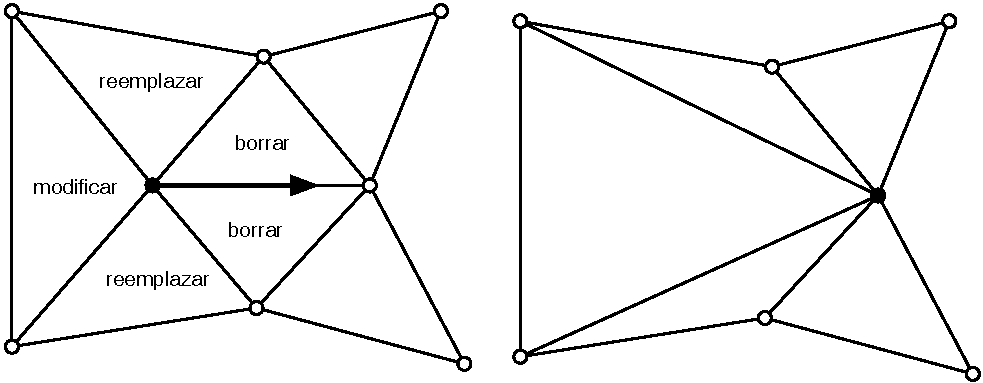
\includegraphics[scale=0.85]{img/img_4.pdf}
\caption{VertexDeletion para caras triangulares}\label{fig:vertex_deletion_t}
\end{figure}

El primer enfoque adoptado para adaptar este algoritmo para cuadril'ateros fue encontrar la analog'ia con el caso de tri'angulos. Se identificaron los mismos actores que en el caso anterior: caras a borrar, caras a modificar, arcos a mantener, etc. y se quiso proceder igual que en el caso triangular, como se explica en la figura \ref{fig:vertex_deletion_q}.\\

\begin{figure}[htp]
\centering
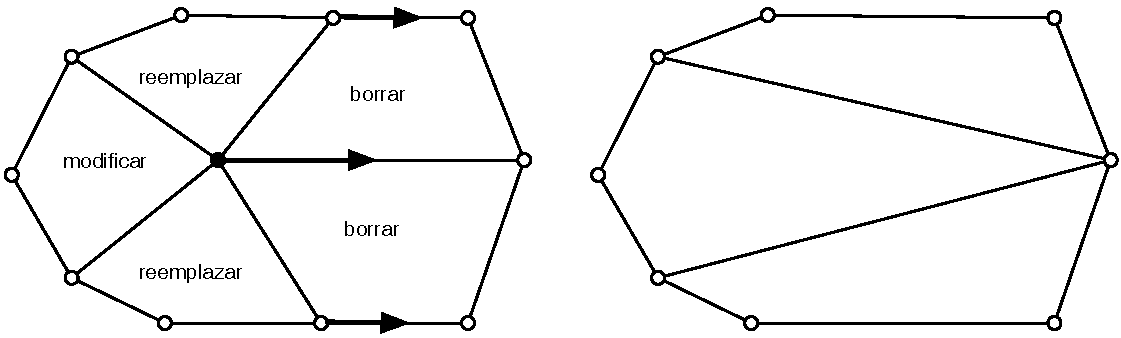
\includegraphics[scale=0.8]{img/img_5.pdf}
\caption{Generalizaci'on VertexDeletion para cuadril'ateros}\label{fig:vertex_deletion_q}
\end{figure}

Sin embargo, este procedimiento no logra los resultados deseados. Para entender lo que ocurre, se puede volver a la explicaci'on intuitiva sobre el procedimiento en una malla triangular: al colapsar un arco en un nodo, a su vez se colapsa en un arco las dos caras adyacentes al arco borrado. Esto no puede ser replicado en un cuadril'atero, pues al colapsar un arco, se forma un tri'angulo. Dejar la malla mixta no es una opci'on pues no permite aplicar ninguno de los algoritmos de modificaci'on de la malla que est'an implementados. La segunda opci'on es colapsar dos arcos, en vez de uno, borrando dos de los nodos pertenecientes a las caras a borrar, como se indica en la figura \ref{fig:vertex_deletion_q_contexto}. En la figura, se muestra una malla inconsistente pues hay un par de arcos en cuya intersecci'on no hay un nodo. Por lo tanto, el borrar estos dos nodos, adicionales con respecto al algoritmo para tri'angulos, conlleva a modificar tambi'en el entorno de esos nodos, lo que hace que el problema deje de ser local y se reproduzca recursivamente, pudiendo no tener soluci'on.\\

\begin{figure}[htp]
\centering
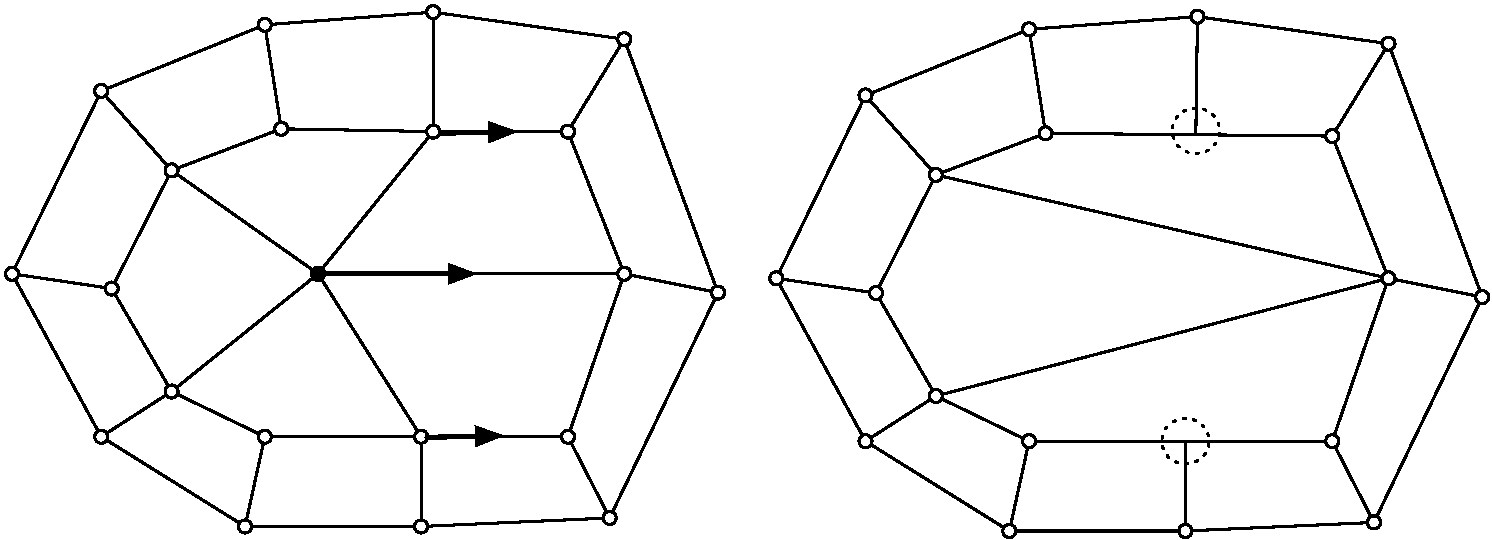
\includegraphics[scale=0.6]{img/img_6.pdf}
\caption{Problema al generalizar VertexDeletion para cuadril'ateros}\label{fig:vertex_deletion_q_contexto}
\end{figure}

Otra forma de entender esto es d'andose cuenta de que el algoritmo para tri'angulos lo que hace es eliminar un nodo y triangular el pol'igono que rodeaba al nodo (el formado por los arcos no incidentes en el nodo, de las caras incidentes en el nodo). Siempre es posible realizar este procedimiento pues siempre es posible triangular un pol'igono \footnote{El algoritmo realiza una triangulaci'on particular que en casos espec'ificos no puede efectuarse, pero se podr'ia hacer otra triangulaci'on}. En cambio, no siempre es posible generar una malla de cuadril'ateros en un pol'igono. De hecho, no se puede generar una malla de cuadril'ateros en un pol'igono cuyo n'umero de arcos es impar.\\

Por otra parte, incluso si s'olo se trabajase con pol'igonos cuyo n'umero de lados es par, igualmente surgen problemas cuando hay arcos adyacentes colineales, lo que se tiene, por ejemplo, al generar la malla de un cilindro. En la figura \ref{fig:arcos_colineales_q} se observa que al borrar el nodo central y generar la malla de cuadril'ateros, quedan colineales arcos adyacentes y pertenecientes a la misma cara, lo que es inconsistente.\\

\begin{figure}[htp]
\centering
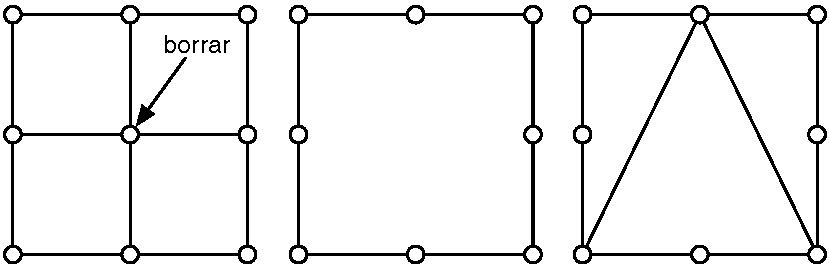
\includegraphics[scale=0.85]{img/img_7.pdf}
\caption{Inconsistencia al generar malla de cuadril'ateros: hay arcos colineales}\label{fig:arcos_colineales_q}
\end{figure}

Una posible soluci'on a este problema es desplazar el nodo que une los arcos colineales de modo de que dejen de serlo. El desplazamiento no puede ser infinitesimal pues se pueden producir errores num'ericos. Este enfoque tiene dos desventajas: puede convertir en c'oncava la cara vecina (si las dos caras se encuentran en la misma situaci'on) y puede generar caras que no pertenezcan a un plano, como se muestra en las figuras \ref{fig:cara_concava_q} y \ref{fig:cara_fuera_plano_q}, respectivamente.\\

\begin{figure}[htp]
\centering
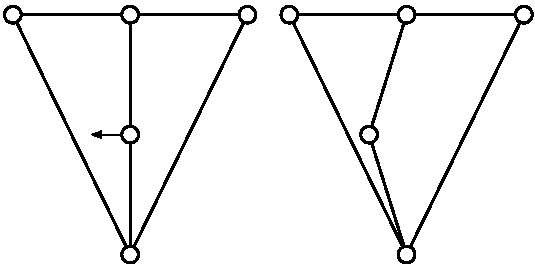
\includegraphics[scale=0.9]{img/img_8.pdf}
\caption{Problema al despazar nodo: una cara es c'oncava y la otra convexa}\label{fig:cara_concava_q}
\end{figure}

\begin{figure}[htp]
\centering
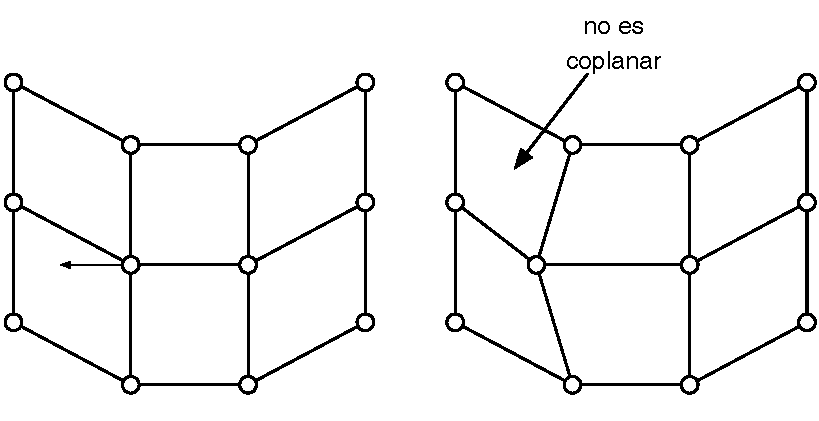
\includegraphics[scale=0.85]{img/img_9.pdf}
\caption{Problema al despazar nodo: Caras dejan de ser coplanares}\label{fig:cara_fuera_plano_q}
\end{figure}

Considerando todo lo anterior, se concluy'o que no es posible utilizar para cuadril'ateros un algoritmo an'alogo al usado para tri'angulos, por lo que se hizo necesario evaluar las implicancias de no contar con este procedimiento para mallas de cuadril'ateros. Para el caso del algoritmo de verificaci'on, se decidi'o implementar un nuevo algoritmo que en vez de colapsar un arco en un punto, colapsa en un punto todas las caras incidentes en el nodo. Para el caso del algoritmo de desrefinamiento, se decidi'o adoptar otra estrategia que no requiere de esta operaci'on. Ambas decisiones se discutir'an en m'as adelante.\\

En la secci'on siguiente se explicar'a el nuevo algoritmo que colapsa una regi'on en un nodo.\\

\section{Algoritmo de colapso de una regi'on en un nodo}

La idea del algoritmo es colapsar en un punto las caras aleda~nas a un nodo. Este procedimiento tiene repercusiones en caras no adyacentes al nodo, por lo que en la pr'actica el algoritmo colapsa una regi'on que rodea al nodo central.\\

El algoritmo detecta el pol'igono que rodea al nodo y desplaza sus v'ertices hacia la posici'on de este nodo central, colapsando el arco que los une y eliminando de esta forma las caras que rodeaban al nodo.\\

En la figura \ref{fig:colapso_region_paso1_t} aparece una malla triangular en donde el pol'igono que se muestra destacado ser'a colapsado en el nodo $n$. En el primer paso, el nodo $n_1$ se desplaza para superponerse al nodo $n$, es decir, se colapsa el arco que une ambos nodos. Al hacer esto, desaparecen las caras $c_1$ y $c_2$. Pero adem'as, este movimiento modifica las caras $c_3$ y $c_6$, vecinas de las caras borradas. Otras dos caras, $c_4$ y $c_5$, aumentan su tama~no.\\

\begin{figure}[htp]
\centering
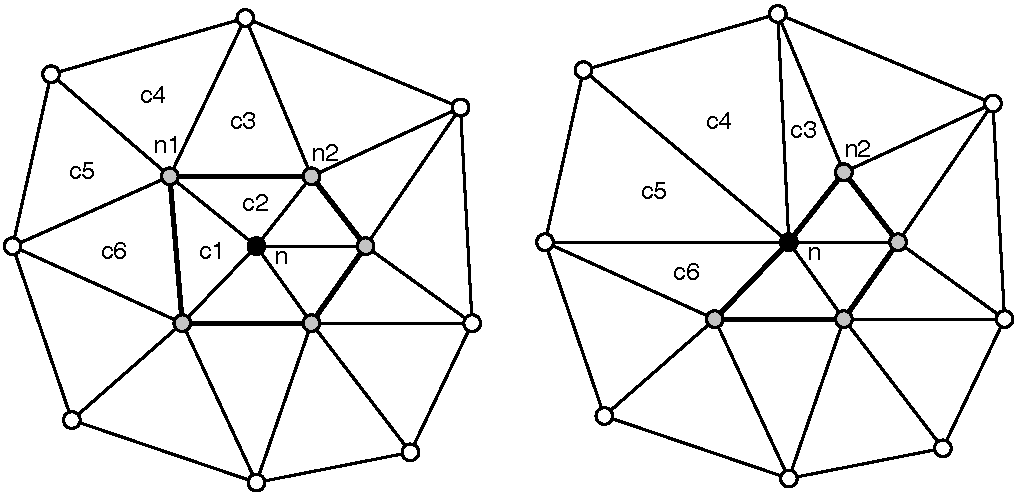
\includegraphics[scale=0.8]{img/img_10.pdf}
\caption{Desplazamiento del nodo $n1$ hacia $n$}\label{fig:colapso_region_paso1_t}
\end{figure}

En el siguiente paso, el nodo $n_2$ se desplazar'a hacia $n$. Esto borrar'a las caras adyacentes al arco colapsado (el que une a $n_2$ con $n$). Repitiendo el procedimiento, se obtendr'a el resultado mostrado en la figura \ref{fig:colapso_region_t}. El algoritmo puede resumirse como la modificaci'on de tres grupos de caras que forman anillos alrededor del nodo: las que lo rodean directamente, las que son vecinas a las anteriores y las que rodean a 'estas 'ultimas. Los dos primeros grupos de caras desaparecen, mientras que las caras del tercero aumentan su 'area, ocupando el espacio que dejaron las caras borradas, lo que se explica en la misma figura. El algoritmo no tiene repercusiones en caras m'as lejanas pues el pol'igono formado por las caras del tercer grupo no cambia, por lo que este algoritmo, al igual que el que colapsa un arco en un nodo, modifica localmente la malla y puede entenderse como una nueva triangulaci'on de un pol'igono que rodea al nodo, salvo que esta vez se considera un pol'igono m'as grande.\\

\begin{figure}[htp]
\centering
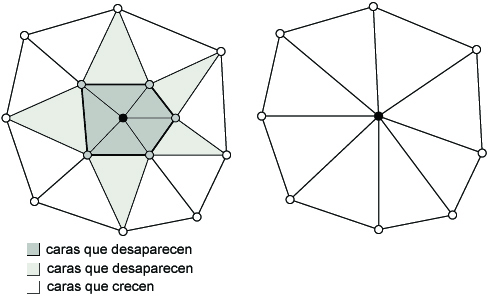
\includegraphics[scale=0.75]{img/img_11.jpg}
\caption{Algoritmo de colapso de una regi'on de tri'angulos}\label{fig:colapso_region_t}
\end{figure}

Para el caso de una malla de cuadril'ateros, el procedimiento es similar: se desplazan hacia el nodo algunos v'ertices del pol'igono que rodea al nodo. Los v'ertices del pol�gono que se desplazan son los que pertenecen a los arcos incidentes en el nodo central (los que en una malla triangular son todos los v'ertices del pol'igono). En este caso, a diferencia del caso triangular, se eliminan s'olo las caras que rodean directamente al nodo. Algunas de las caras que forman el segundo anillo alrededor del nodo aumentan su 'area, ocupando el espacio dejado por las caras borradas, como se muestra en la figura \ref{fig:colapso_region_q}.\\

\begin{figure}[htp]
\centering
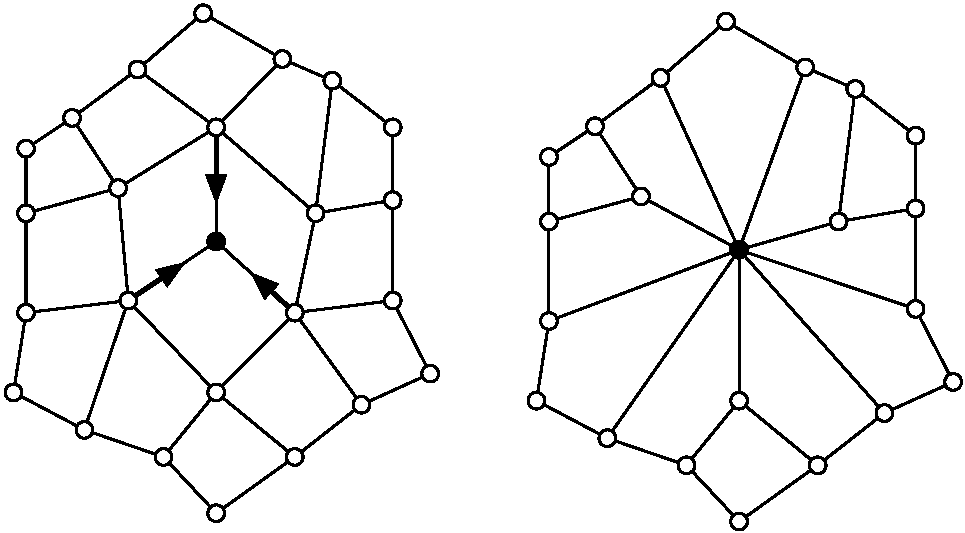
\includegraphics[scale=0.8]{img/img_12.pdf}
\caption{Algoritmo de colapso de una regi'on de cuadril'ateros}\label{fig:colapso_region_q}
\end{figure}

En el algoritmo explicado en la secci'on anterior, el que una de las caras que se borran tuviera dos caras vecinas que adem'as son vecinas entre ellas produce un caso degenerado. Para evitar que ocurra, si la malla est'a en esa situaci'on, el procedimiento no se aplica.\\

En este nuevo algoritmo, este caso es an'alogo en el caso de mallas triangulares. Para el caso de mallas de cuadril'ateros, el algoritmo puede ser aplicado en este caso, pero genera cuadril'ateros c'oncavos. En la figura \ref{fig:colapso_region_rara_q} se observa que la cara $c_1$ ser'a borrada y dos de sus caras vecinas, $c_2$ y $c_3$, son vecinas entre ellas. Al desplazar los nodos $n_1$ y $n_2$ hacia el nodo $n$, los arcos $a_1$ y $a_2$ se juntar'an, por lo que las caras $c_2$ y $c_3$ compartir'an dos arcos, lo que hace que o bien esos dos arcos son colineales, en cuyo caso estamos frente a dos cuadril'ateros degenerados (tienen tres lados), o bien uno de los cuadril'ateros es convexo y el otro c'oncavo (los arcos forman dos 'angulos, cada uno perteneciente a una de las caras, si uno de los 'angulos mide menos de 180�, el otro debe medir m'as de 180�), como se muestra tambi'en en la figura.\\

\begin{figure}[htp]
\centering
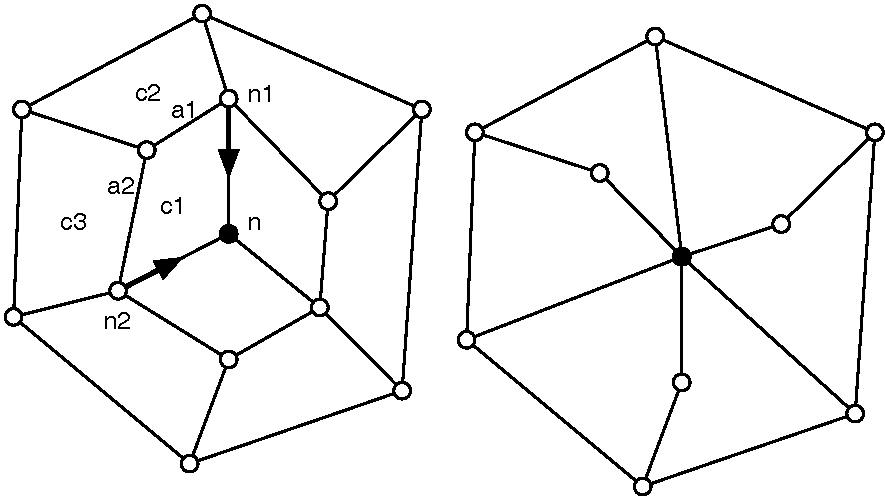
\includegraphics[scale=0.8]{img/img_13.pdf}
\caption{Aparici'on de caras c'oncavas al colapsar regi'on}\label{fig:colapso_region_rara_q}
\end{figure}

Tener caras c'oncavas es una desventaja, pero no hace que se descarte el algoritmo. De hecho, se considera que modificar la malla para que deje de tener caras c'oncavas es una forma de mejorar la calidad de la malla, por lo que es un buen trabajo futuro incorporar algoritmos que trabajen en ese sentido.\\

En particular, se sugieren dos algoritmos de mejoramiento de la malla que abordan el problema. El primero de ellos consiste en 
reconocer pares de cuadril'ateros vecinos, que comparten un solo arco, tales que al reemplazar el arco com'un por otro de los dos posibles (\emph{flipping de arcos}), ambos cuadril'ateros queden convexos. En la figura \ref{fig:mejoramiento_q} se muestra el resultado de aplicar dos veces esta idea, a partir de la malla producida al colapsar la regi'on. Uno de los tres casos de concavidad del ejemplo no pudo ser solucionado por el algoritmo.\\

\begin{figure}[htp]
\centering
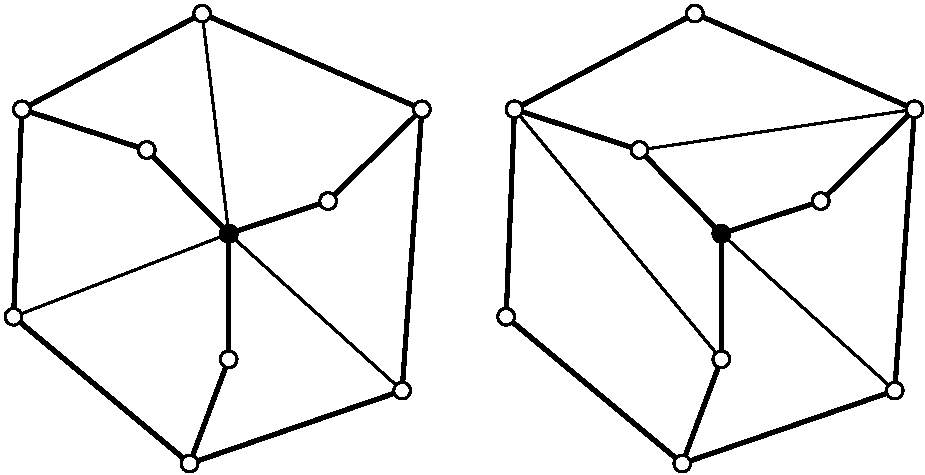
\includegraphics[scale=0.8]{img/img_14.pdf}
\caption{\emph{Flipping} de arcos para mejorar calidad de la malla}\label{fig:mejoramiento_q}
\end{figure}

Otro algoritmo posible consiste en reconocer pares de cuadril'ateros que comparten dos arcos y eliminar esos dos arcos y el nodo que los une. Como los cuadril'ateros compart'ian dos arcos, cada uno de ellos tiene otros dos arcos. La uni'on se los dos pares de arcos sobrevivientes forma tambi'en un cuadril'atero. Este enfoque mejora la calidad de la malla y tambi'en la desrefina, lo que no siempre es deseable.\\

Si se tiene un caso como el mostrado en la figura \ref{fig:colapso_region_rara_q}, en que todas las caras a borrar tienen caras vecinas que son vecinas entre s�, aplicar el algoritmo de colapso de la regi�n y posteriormente aplicar este segundo algoritmo de mejoramiento produce un resultado similar al obtenido aplicando el algoritmo de colapso en una malla de tri'angulos.\\ %(comparar las figuras figura ***2 y figura ***5).\\

\subsection{Detalle de la implementaci'on y discusi'on}

Para aplicar el algoritmo antes explicado, tanto para mallas de tri'angulos como para el caso de cuadril'ateros, se necesita que la malla cumpla con las condiciones descritas en los ejemplos, esto es, que se puedan reconocer dos bordes alrededor del nodo a colapsar, en el caso de tri'angulos, y uno en el caso de cuadril'ateros.\\

Durante el testeo de los m'etodos implementados se encontraron casos en que la malla se encontraba en una configuraci'on distinta a la que se esperaba, lo que produc'ia que los m'etodos fallaran. Por ejemplo, en la malla triangular, el caso en que dos caras vecinas y adyacentes al nodo central comparten una tercera cara vecina.\\

La implementaci'on de estos m'etodos result'o m'as dificultosa de lo inicialmente estimado, debido a la necesidad de actualizar las referencias cruzadas entre nodos, arcos y caras. La implementaci'on es muy sensible al orden en que se hacen las actualizaciones, pues no puede perderse informaci'on que luego se necesitar'a para hacer una posterior actualizaci'on.\\

Para evitar complejizar a'un m'as la implementaci'on, se opt'o por crear una copia de los elementos de la malla (nodos, arcos y caras) antes de modificarla. Entonces, en vez de chequear a priori si se cumplen las precondiciones del m'etodo, se chequea cuando 'estas son relevantes y, en caso de no cumplirse, se aborta el colapso y se restituye la malla a su estado original.\\

Esta decisi'on tiene un costo en eficiencia, tanto en tiempo como en espacio, pero se considera apropiada para la situaci'on y la aplicaci'on sigue corriendo con un uso de recursos aceptable, incluso con mallas de decenas de miles de nodos.\\

Para llevar a cabo el respaldo de los elementos de la malla, se implement'o en las clases \emph{Nodos}, \emph{Arcos} y \emph{Caras} el m'etodo \emph{clone} que llama al constructor de copia, implementado para este fin, el que tiene visibilidad protegida. Adem'as, se implement'o tambi'en el m'etodo \emph{clone} en las clases \emph{Nodo}, \emph{Arco} y \emph{Cara}. La soluci'on adoptada \cite{clone} consiste en hacer una copia profunda de los contenedores, es decir, crear no s'olo el contenedor, sino tambi'en los objetos contenidos. La utilizaci'on de los m'etodos \emph{clone} en las clases de los objetos contenidos es una aplicaci'on del patr'on \emph{Prototype} y permite delegar en las subclases la creaci'on de la copia de los objetos que son instancia de esas subclases. Esto permite, por ejemplo, que la clase \emph{Caras} se clone correctamente, es decir, respetando el tipo din'amico de las caras que contiene (caras generales, tri'angulos o cuadril'ateros), sin necesidad de que tal clase conozca esa informaci'on.\\

\section{Algoritmos de verificaci'on}

Se extendi'o a mallas de cuadril'ateros el algoritmo \emph{Verificaci'on de Nodos Vecinos}.\\

La primera parte de la adaptaci'on consisti'o en generalizar la forma en que el algoritmo detecta que existir'a una colisi'on al desplazar un nodo. El algoritmo crea un pseudo-cilindro en el que la base inferior es el pol'igono que rodea a un nodo central y la base superior se forma por las posiciones futuras de los v'ertices del pol'igono. Es decir, los arcos verticales del cilindro son las trayectorias de los nodos que forman el pol'igono. Luego detecta si la trayectoria del nodo central chocar'a con alguna de las caras del cilindro. Se generaliz'o la forma en que el algoritmo genera este cilindro, pues originalmente la implementaci�n era v�lida s�lo para el caso de mallas triangulares.\\

La segunda parte de la adaptaci'on se relaciona con c'omo el algoritmo soluciona una futura colisi'on. El primer intento consiste en modificar la trayectoria del nodo central. Si esto falla, entonces elimina el nodo central. Es aqu'i donde el algoritmo ocupa el m'etodo \emph{VertexDeletion} que colapsa un arco en un nodo y que, como se explic'o anteriormente, no es posible generalizar para mallas de cuadril'ateros.\\

La estrategia adoptada entonces fue crear un nuevo algoritmo de verificaci'on (\emph{VerificacionNodosVecinosColapsoRegion}), v'alido para mallas de tri'angulos y para mallas de cuadril'ateros. El algoritmo act'ua igual que el anterior salvo en el momento en que la colisi'on no pudo ser solucionada mediante el cambio de la trayectoria del nodo central.\\

Si no se pudo solucionar la colisi'on, lo que se hace es colapsar en el nodo central la regi'on que rodea a tal nodo. La intuici'on que explica esto es que el desplazamiento de los nodos corresponde al crecimiento del tronco del 'arbol. Si pese a cambiar la trayectoria del nodo sigue produci'endose la colisi'on, entonces no es responsabilidad del nodo, sino de las trayectorias de los nodos vecinos. Es decir, existe un conjunto de c'edulas del 'arbol (caras de la malla) que interfieren entre s'i, por lo que se eliminan todas ellas, absorbidas por las c'elulas que las rodean y se mantiene el nodo.\\

Esta soluci'on es m'as sim'etrica que la original, que colapsa un arco cualquiera de la regi'on problem'atica.

Por lo tanto el nuevo algoritmo de verificaci'on y soluci'on de colisiones utiliza el algoritmo de colapso de una regi'on en un nodo, explicado en la secci'on anterior.\\

Finalmente, los resultados obtenidos con este algoritmo no fueron totalmente satisfactorios en el caso de mallas irregulares. Por ejemplo, se cuenta con una malla que modela la superficie de un moai. Este ejemplo constituye el peor caso que se tuvo para probar el algoritmo, pues la cara del moai presenta irregularidades (la nariz y la hendidura de los ojos) que hacen que al deformarse se produzcan muchas colisiones, varias que no pueden solucionarse corrgiendo la trayectoria de nodo central, por lo que el algoritmo de colapso debe aplicarse reiteradamente en una zona peque~na.\\

En el caso de esa malla, se observ'o que se sobrecargan unos pocos nodos de las regiones cr'iticas, pues cada vez que se colapsa una regi'on, el nodo central hereda los arcos sobrevivientes de las caras borradas. Al repetirse la operaci'on en otro nodo cercano, este nuevo nodo recibe los arcos del nodo anterior, que ya acumulaba los arcos heredados en los colapsos anteriores.\\

Se cree que el comportamiento del algoritmo podr'ia mejorar si se le agrega un criterio para que el colapso se efect'ue s'olo si las caras que se colapsan son peque~nas. Esta condici'on modela mejor el comportamiento de las c'elulas del 'arbol, que son absorbidas por sus vecinas cuando son alcanzan un tama~no peque~no.\\

Sin embargo, al probar el algoritmo en mallas m'as regulares, que se condicen mejor con la forma cil'indrica del tronco de un 'arbol, los resultados fueron m'as satisfactorios.\\

\section{Algoritmos de desrefinamiento}

El algoritmo de desrefinamiento \emph{Edge Collapse} que est'a implementado para mallas triangulares en la aplicaci'on del legado, recorre la malla y, para cada cara que no cumple el criterio de detenci'on, colapsa el menor de sus arcos, eliminando las dos caras adyacentes al arco. Para ello utiliza el m'etodo \emph{VertexDeletion} que no es extendible a mallas de cuadril'ateros.\\

Un enfoque posible es utilizar el nuevo m'etodo que colapsa una regi'on en un nodo. El problema de esto es que el m'etodo elimina todas las caras que rodean un nodo, es decir, no se puede asegurar que s'olo se eliminan las caras peque~nas. El algoritmo original tiende a eliminar s'olo las caras peque~nas pues de cada cara suficientemente peque~na (seg'un el criterio elegido), elimina su arco m'as peque~no, con lo que adem'as de eliminar la cara que cumple el criterio, elimina la otra cara adyacente al arco, pero como el arco es peque~no (el menor arco de una cara peque~na debe ser peque~no), la segunda cara tambi'en debe serlo.\\

Por lo tanto, si bien es factible hacer un algoritmo de desrefinamiento basado en la eliminaci'on de regiones de la malla, probablemente su resultado no ser'a satisfactorio pues elimina demasiadas caras, incluso si se tiene la precauci'on  de no aplicar el m'etodo de eliminaci'on sobre todos los nodos, por ejemplo, excluyendo los nodos que forman el borde de las regiones que ya han sido desrefinadas.\\

Entonces, el enfoque elegido es triangular la malla de cuadril'ateros, a~nadiendo diagonales en los cuadril'ateros; utilizar el algoritmo de desrefinamiento para mallas triangulares y finalmente hacer que la malla vuelva a ser de cuadril'ateros.\\

Esta estrategia no fue implementada, pero s'i lo fueron los pasos que la componen. Por lo tanto, el usuario puede reproducir este proceso en la aplicaci'on. Hay que tener especial cuidado en informarle al usuario que al convertir una malla de tri'angulos en una de cuadril'ateros y viceversa, la malla se refina. Por lo tanto, debe considerar esta informaci'on al elegir los criterios que determinan qu'e tanto se desrefina la malla intermedia de tri'angulos.\\

\section{Algoritmo para convertir una malla de tri'angulos en malla de cuadril'ateros}

El algoritmo consiste en dividir cada cara triangular en tres cuadril'ateros, insertando un nodo en el centro del tri'angulo y un nodo en cada arista, como se muestra en la figura \ref{fig:cuadrangular}.\\

\begin{figure}[htp]
\centering
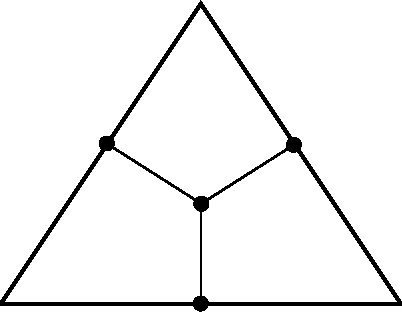
\includegraphics[scale=0.7]{img/cuadrangular.pdf}
\caption{Cuadrangulaci'on de una cara triangular}\label{fig:cuadrangular}
\end{figure}

Para llevar a cabo el proceso, se recorren las caras de la malla y se dividen sus aristas, creando nuevas caras. Es necesario considerar que al dividir una arista (es decir, eliminarla y crear otras dos) se afecta no s'olo la cara sobre la cual se est'a iterando, sino que tambi'en la cara vecina a 'esta, a trav'es de la arista modificada. Por lo tanto, fue necesario dise~nar un sistema para guardar, para cada arista original, las dos aristas creadas y el nuevo nodo que las une, de manera que al recorrer las aristas de la cara original, 'estas se dividan s'olo si no hab'ian sido divididas anteriormente.\\

Como en todos los algoritmos que modifican la malla, hay que tener tambi'en especial cuidado en actualizar las referencias cruzadas entre los elementos de la malla: nodos, arcos y caras.\\

Para incorporar esta nueva funcionalidad en la aplicaci'on, se segui'o el dise~no existente, es decir, se cre'o una clase que implementa la interfaz \emph{Comando} y se agreg'o una jerarqu'ia para agregar nuevas implementaciones de este algoritmo, lo que corresponde a la aplicaci'on de los patrones \emph{Command} y \emph{Strategy}, respectivamente.\\

Adem'as, se cre'o una jerarqu'ia de clases para el criterio de calcular el centro del tri'angulo. Se implement'o la clase que lo calcula como el baricentro, pero podr'ian agregarse nuevos criterios, como calcularlo como el incentro del tri'angulo.\\

Finalmente, se agregaron los botones en la interfaz y el cuadro de di'alogo para seleccionar el algoritmo y criterio elegidos.\\

\section{Algoritmo para convertir una malla de cuadril'ateros en malla de tri'angulos}

Se desarroll'o un algoritmo simple para convertir cada cuadril'atero de la malla en dos tri'angulos, agregando una diagonal.\\

Se tomaron las mismas consideraciones del algoritmo inverso en cuanto a la actualizaci'on de las referencias cruzadas.\\

Igualmente, se aplicaron los patrones \emph{Command} y \emph{Strategy} y se modific'o la interfaz para incorporar esta nueva funcionalidad.\\

\section{Correcci'on de errores}

Durante el desarrollo del trabajo de esta memoria se encontraron errores heredados de la aplicaci'on del legado. Ellos ten'ian distintos niveles de impacto en la aplicaci'on, pero s� impactaron de forma importante el desarrollo de 'esta, pues en general eran errores que no se detectan en los casos de prueba usuales, por lo que en un principio fueron atribuidos a los cambios introducidos durante este desarrollo y se utiliz'o una gran cantidad de tiempo en hacer un seguimiento de los cambios para concluir finalmente que eran errores heredados.\\

Esta situaci'on se produjo porque al cambiar cada parte de la aplicaci'on se prob'o su funcionamiento fabricando mallas peque~nas de forma de poder garantizar que la malla generada era una instancia v'alida (revisando sus variables de instancia).\\

Se considera que fue valioso realizar este chequeo minucioso, pese al tiempo que utiliz�, pues permiti� detectar errores que no se notaban al visualizar la malla, lo que explica que no hayan sido corregidos cuando se desarroll'o la aplicaci'on del legado.\\

A continuaci'on se explican los errores encontrados y solucionados:

\begin{description}

\item[Ejecuci'on en modo \emph{debug}:] Uno de los m'etodos utilizados para graficar la malla chequeaba una precondici'on que generalmente no se cumpl'ia. Por lo tanto, al ejecutar la aplicaci'on en modo \emph{debug} (con las instrucciones \emph{assert} activadas), el programa se ca'ia. Este error no se detectaba al ejecutar la aplicaci'on en modo \emph{release}.

\item[Visualizaci'on la malla:] Al cargar una malla en que todos los nodos ten'ian concentraci'on nula, las caras se graficaban de color negro, en vez del color azul esperado. Esto se debe a que el color de los nodos es proporcional a la concentraci'on del nodo con respecto a la m'axima concentraci'on de la malla. No se consideraba el caso en que 'ese m'aximo era cero, por lo que se produc'ia una divisi'on por cero.
\item[Deformaci'on de la malla:] En el c'alculo de las normales de las caras faltaba normalizar el vector. Estas normales se utilizan para calcular la normal de los nodos, la que define la direcci'on del desplazamiento del nodo. Por lo tanto, el error hac'ia que la deformaci'on de la malla no fuera la deseada.

Adem'as, se encontr'o otro error al calcular la normal de los nodos. 'Esta se calculaba como la suma de las normales incidentes en el nodo. En el ejemplo de la figura \ref{fig:malla_normales} se muestra una malla de seis caras triangulares, donde todas las diagonales van desde el nodo superior izquierdo al nodo inferior derecho. Cada nodo de la malla forma parte de tres caras. Dada la simetr'ia del ejemplo, se espera que las normales de los nodos sean radiales y que los nodos pertenecientes a un mismo arco vertical tengan las mismas normales. Sin embargo no se obten'ia eso, pues se consideraban de igual forma las tres normales de las caras, por lo que un vector se sumaba dos veces. Esto se corrigi'o considerando que el peso de cada cara en el nodo es proporcional al 'angulo que forma la cara en ese nodo.

\begin{figure}[htp]
\centering
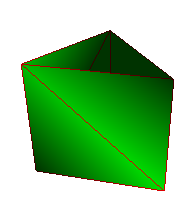
\includegraphics[scale=0.8]{img/malla_normales.png}
\caption{Malla de seis caras triangulares}\label{fig:malla_normales}
\end{figure}

\item[Consistencia de la malla:] En el m'etodo que estaba implementado para generar una malla de cuadril'ateros a partir de un archivo de formato \emph{Matlab}, se calculaba mal uno de los 'indices de los arcos que forman la cara. Esto hac'ia que la cara registrara que estaba formada por un arco que no informaba que fuera parte de esa cara, pues efectivamente no lo era. Este error no se notaba al visualizar la malla, pues ah'i se ocupa la informaci'on de los nodos que componen la cara y esa informaci'on estaba correcta. Sin embargo, en m'etodos que recorren los arcos de la cara el error se hac�a presente. Se solucion'o el error y adem'as se modific'o un m'etodo que chequea la consistencia de la malla, para que revisara tambi'en que todas las relaciones entre elementos de la malla sean sim'etricas, es decir, en ambos sentidos. Por ejemplo, si un arco se relaciona con una cara, la cara tambi'en se debe relacionar con el arco.

\item[Detecci'on de colisiones:] En el algoritmo \emph{Verificaci'on de Nodos Vecinos} que detecta y soluciona las colisiones al deformar la malla no se cubr�a el caso en que algunos de los nodos de la malla no se desplazaran (tuvieran una concentraci'on nula), por lo que la aplicaci'on se ca'ia al deformar la malla ocupando ese algortimo. 

\end{description}
\chapter{Conclusiones}
�stas son las conclusiones.
\bibliographystyle{plain}
\bibliography{refs}
\begin{appendix2}
\section{Formatos de archivos de entrada y salida}

\begin{figure}[htp]
\centering
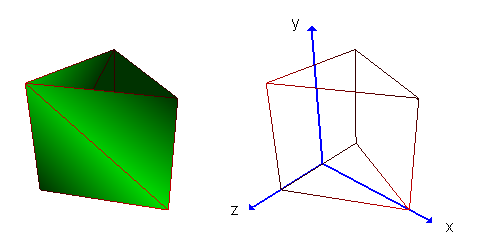
\includegraphics[scale=0.9]{img/malla_formato.png}
\caption{Malla que se representar'a en distintos formatos}\label{fig:malla_formato}
\end{figure}

La aplicaci'on importa y exporta mallas en distintos formatos. A continuaci'on se explican los formatos utilizados. Esta informaci'on se obtuvo analizando el c'odigo de la aplicaci'on y los archivos de mallas y se registra aqu'i pues se considera que ser'a de ayuda para futuras extensiones de la aplicaci'on.\\

Se ejemplificar'an los formatos con la malla mostrada en la figura \ref{fig:malla_formato}.\\

\begin{description}
\item[Comsol - Extensi'on cms\_1:] El archivo se divide en dos secciones: coordenadas y elementos. La primera l'inea indica el inicio de la secci'on de coordenadas. A partir de la segunda l'inea, en cada l'inea se encuentran las coordenadas \emph{x,y,z} de un nodo de la malla. Luego, hay una l'inea que indica el inicio de la secci'on de elementos y posteriormente en cada l'inea se encuentra la informaci'on de una cara. La cara se especifica indicando los 'indices 1-basados de los nodos que la componen, seg'un el orden en que los nodos fueron especificados en la primera secci'on.

\texttt{
\begin{tabular}{|l|} \hline
Archivo malla.cms\_1 \\ \hline
\% Coordinates \\
10    0   0\\
0    0   5\\
0    0  -5\\
10   10   0\\
0   10   5\\
0   10  -5\\
\% Elements (triangular)\\
2  5  1\\
5  4  1\\
3  6  2\\
6  5  2\\
1  4  3\\
4  6  3\\ \hline
\end{tabular}
}

\item[Matlab - Extensi'on txt:] Este formato se utiliza s'olo para mallas tubulares (es decir, con anillos alrededor de una m'edula). Al cargar el archivo, el usuario indica el n'umero de anillos de la malla y la cantidad de puntos por cada anillo. El archivo se divide en cuatro secciones. Primero est'an las coordenadas \emph{x} de todos los nodos, luego las \emph{z} y las \emph{y}. Finalmente, est'an las concentraciones de los nodos. No son relevantes los saltos de l'inea en el archivo, pero para un mejor entendimiento, se tiene la convenci'on de que cada l'inea del archivo tiene los datos de un anillo de la malla.

En este formato no existe una secci�n donde se indique qu'e nodos forman cada cara, sino que esto se deduce de la ubicaci'on de los nodos en los anillos. Es por esto que el mismo archivo puede representar una malla de tri'angulos o de cuadril'ateros, dependiendo de c'omo se unen los nodos mediante arcos.

\texttt{
\begin{tabular}{|l|} \hline
Archivo malla.txt \\ \hline
10 0 0\\
10 0 0\\
0 5 -5\\
0 5 -5\\
0 0 0\\
10 10 10\\
1 1 1\\
0 0 0\\ \hline
\end{tabular}
}

\item[nxyzu - Extensi'on txt:] La informaci'on de la malla se divide en cuatro archivos: \emph{nx}, \emph{ny}, \emph{nz} y \emph{u}. Por convenci'on, al final del nombre del archivo se indica de cu'al de los cuatro tipos es el archivo. Cada archivo tiene tres secciones. Las primeras dos secciones son iguales al formato \emph{Comsol} y son las mismas en los cuatro archivos. La tercera secci'on tiene las coordenadas del vector normal y la concentraci'on de cada nodo. En el archivo \emph{nx} est'a la coordenada \emph{x} de las normales de los nodos, en el mismo orden en que se listan los nodos en la primera secci'on. Es an'alogo para \emph{ny} y \emph{nz}. En el archivo \emph{u} est'a la concentraci'on de hormona en el nodo, es decir, el m'odulo del vector desplazamiento del nodo.

\texttt{
\begin{tabular}{|l|l|} \hline
Archivo malla\_nx.txt & Archivo malla\_ny.txt \\ \hline
\% Coordinates & \% Coordinates \\
10    0   0 & 10    0   0 \\
0    0   5 & 0    0   5 \\
0    0  -5 & 0    0  -5 \\
10   10   0 & 10   10   0 \\
0   10   5 & 0   10   5 \\
0   10  -5 & 0   10  -5 \\
\% Elements (triangular) & \% Elements (triangular) \\
1  5  2 & 1  5  2 \\
1  4  5 & 1  4  5 \\
2  6  3 & 2  6  3 \\
2  5  6 & 2  5  6 \\
3  4  1 & 3  4  1 \\
3  6  4 & 3  6  4 \\
\% Data (nx) & \% Data (ny)\\
1.000000 & 0.00000\\
-0.525731 & 0.00000\\
-0.525731 & 0.00000\\
1.000000 & 0.00000\\
-0.525731 & 0.00000\\
-0.525731 & 0.00000\\\hline
\end{tabular}
}

\texttt{
\begin{tabular}{|l|l|} \hline
Archivo malla\_nz.txt & Archivo malla\_u.txt \\ \hline
\% Coordinates & \% Coordinates \\
10    0   0 & 10    0   0 \\
0    0   5 & 0    0   5 \\
0    0  -5 & 0    0  -5 \\
10   10   0 & 10   10   0 \\
0   10   5 & 0   10   5 \\
0   10  -5 & 0   10  -5 \\
\% Elements (triangular) & \% Elements (triangular) \\
1  5  2 & 1  5  2 \\
1  4  5 & 1  4  5 \\
2  6  3 & 2  6  3 \\
2  5  6 & 2  5  6 \\
3  4  1 & 3  4  1 \\
3  6  4 & 3  6  4 \\
\% Data (nz) & \% Data (u)\\
0.000000 & 1.000000\\
0.850651 & 1.000000\\
-0.850651 & 1.000000\\
0.000000 & 0.000000\\
0.850651 & 0.000000\\
-0.850651 & 0.000000\\
\hline
\end{tabular}
}

\item[Geomview - Extensi'on off:] Las primeras dos l'ineas del archivo son informativas, la primera indica que se trata de un archivo en formato \emph{off} y la segunda indica el n'umero de nodos, caras y arcos de la malla. El n'umero de arcos no se ocupa, sino que se deduce de la topolog'ia de la malla. Las siguientes l'ineas contienen las coordenadas de los nodos y las 'ultimas l'ineas corresponden a las caras. El primer n'umero de la l'inea de una cara indica el n'umero de lados de la cara, luego se indican los 'indices 0-basados de los nodos que componen la cara. Opcionalmente se puede indicar tambi'en el color de la cara en formato \emph{RGB}. La aplicaci'on lee y almacena el color de la cara, si es proporcionado, pero no lo utiliza al graficar la malla. En el ejemplo, la mitad de las caras tienen color rojo y la otra mitad verde.

\texttt{
\begin{tabular}{|l|} \hline
Archivo malla.off \\ \hline
OFF\\
6 6 12\\
10    0   0\\
0    0   5\\
0    0  -5\\
10   10   0\\
0   10   5\\
0   10  -5\\
3 0 4 1 1 0 0\\
3 0 3 4 1 0 0\\
3 1 5 2 1 0 0\\
3 1 4 5 0 1 0\\
3 2 3 0 0 1 0\\
3 2 5 3 0 1 0\\ \hline
\end{tabular}
}

\item[Debug - Extensi'on mll:] Este formato se utiliza para depurar la aplicaci'on. En 'el se muestra toda la informaci'on de la malla. La primera l'inea indica que se que se trata de un archivo de formato \emph{Debug}. La segunda l'inea indica el n'umero de nodos, caras y arcos de la malla. La l'inea siguiente es similar a la anterior, pero se limita a los nodos, caras y arcos v'alidos (es decir, sin incluir los elementos borrados). A partir de la cuarta l'inea se listan los nodos, indicando las caras y arcos a los que pertenece el nodo, la normal y la concentraci'on. Luego se listan los arcos, indicando los nodos que lo forman y las caras de las que forma parte. Finalmente se listan las caras de la malla, junto con el n'umero de lados de la cara; los arcos que la conforman, los que a su vez indican los nodos que los conforman; la normal de la cara y la concentraci'on de la cara.

En el ejemplo, por razones de espacio, se cambiaron las palabras \emph{Nodos}, \emph{Nodo}, \emph{Caras}, \emph{Cara}, \emph{Arcos}, \emph{Arco}, \emph{Normal} y \emph{Concentracion} por \emph{N}s, \emph{N}, \emph{Cs}, \emph{C}, \emph{As}, \emph{A}, \emph{Nor} y \emph{Con}, respectivamente.

\begin{small}
\texttt{
\begin{tabular}{|l|} \hline
Archivo malla.mll \\ \hline
MLL (Debug file)\\
6 6 12\\
6 6 12\\
N\{0\}=(10,0,0) Cs\{0,1,4\} As\{0,2,3,10\} Nor=(1,0,0) Con=\{1\} \\
N\{1\}=(0,0,5) Cs\{0,2,3\} As\{1,2,5,7\} Nor=(-0.525,0,0.850) Con=\{1\} \\
N\{2\}=(0,0,-5) Cs\{2,4,5\} As\{6,7,9,10\} Nor=(-0.525,0,-0.850) Con=\{1\} \\
N\{3\}=(10,10,0) Cs\{1,4,5\} As\{3,4,9,11\} Nor=(1,0,0) Con=\{1\} \\
N\{4\}=(0,10,5) Cs\{0,1,3\} As\{0,1,4,8\} Nor=(-0.525,0,0.850) Con=\{1\} \\
N\{5\}=(0,10,-5) Cs\{2,3,5\} As\{5,6,8,11\} Nor=(-0.525,0,-0.850) Con=\{1\} \\
A\{0\} Ns\{0,4\} Cs\{0,1\} \\
A\{1\} Ns\{4,1\} Cs\{0,3\} \\
A\{2\} Ns\{1,0\} Cs\{0,-1\} \\
A\{3\} Ns\{0,3\} Cs\{1,4\} \\
A\{4\} Ns\{3,4\} Cs\{1,-1\} \\
A\{5\} Ns\{1,5\} Cs\{2,3\} \\
A\{6\} Ns\{5,2\} Cs\{2,5\} \\
A\{7\} Ns\{2,1\} Cs\{2,-1\} \\
A\{8\} Ns\{4,5\} Cs\{3,-1\} \\
A\{9\} Ns\{2,3\} Cs\{4,5\} \\
A\{10\} Ns\{0,2\} Cs\{4,-1\} \\
A\{11\} Ns\{5,3\} Cs\{5,-1\} \\
C\{0\} 3 Ns\{0,4,1\} As\{0:0-->4,1:4-->1,2:1-->0\} Nor=(0.447,0,0.894) Con=3 \\
C\{1\} 3 Ns\{0,3,4\} As\{3:0-->3,4:3-->4,0:0-->4\} Nor=(0.447,-0,0.894) Con=3 \\
C\{2\} 3 Ns\{1,5,2\} As\{5:1-->5,6:5-->2,7:2-->1\} Nor=(-1,-0,-0) Con=3 \\
C\{3\} 3 Ns\{1,4,5\} As\{1:4-->1,8:4-->5,5:1-->5\} Nor=(-1,0,0) Con=3 \\
C\{4\} 3 Ns\{2,3,0\} As\{9:2-->3,3:0-->3,10:0-->2\} Nor=(0.447,0,-0.894) Con=3 \\
C\{5\} 3 Ns\{2,5,3\} As\{6:5-->2,11:5-->3,9:2-->3\} Nor=(0.447,0,-0.894) Con=3 \\\hline
\end{tabular}
}
\end{small}

\end{description}

\end{appendix2}
\end{document}